\documentclass[12pt]{article}
\usepackage[utf8]{inputenc}
\usepackage{parskip}
\usepackage{url}
\usepackage{graphicx}
\usepackage{float}
\usepackage{microtype} % Slightly tweak font spacing for aesthetics
\usepackage{hyperref}

\usepackage{menukeys} % Used to provide graphical key combinations, menu items and file paths.

% Start document here

\begin{document}

% Cover page
\begin{center}

\includegraphics[scale=0.7]{images/logo.jpg}
\end{center}

\renewcommand\thepage{}

% Title page
\begin{titlepage}
\begin{centering}
\huge{Murcs' User Guide}

\vspace{1cm}

\large{Last updated \\ \today}

\vfill

\large{Created by Suspiciously Willing Software \textregistered}

\end{centering}
\thispagestyle{empty}
\end{titlepage}



% Copyright page

Copyright \textcopyright 2015 Daniel van Wichen, Dion Woolley, Haydon Baddock, James Fairbairn, Jay Harris, Matthew Knox

Permission is hereby granted, free of charge, to any person obtaining a copy
of this software and associated documentation files \(the "Software"\), to deal
in the Software without restriction, including without limitation the rights
to use, copy, modify, merge, publish, distribute, sublicense, and/or sell
copies of the Software, and to permit persons to whom the Software is
furnished to do so, subject to the following conditions:

The above copyright notice and this permission notice shall be included in
all copies or substantial portions of the Software.

THE SOFTWARE IS PROVIDED "AS IS", WITHOUT WARRANTY OF ANY KIND, EXPRESS OR
IMPLIED, INCLUDING BUT NOT LIMITED TO THE WARRANTIES OF MERCHANTABILITY,
FITNESS FOR A PARTICULAR PURPOSE AND NONINFRINGEMENT. IN NO EVENT SHALL THE
AUTHORS OR COPYRIGHT HOLDERS BE LIABLE FOR ANY CLAIM, DAMAGES OR OTHER
LIABILITY, WHETHER IN AN ACTION OF CONTRACT, TORT OR OTHERWISE, ARISING FROM,
OUT OF OR IN CONNECTION WITH THE SOFTWARE OR THE USE OR OTHER DEALINGS IN
THE SOFTWARE.

\thispagestyle{empty}

% A preface, containing details of related documents and information on how to navigate the user guide
\section{Preface}

% A contents page
\tableofcontents

% A list of requirements you need to meet to run the applications
\section{Requirements}

Murcs requires Java 8 u40 or later.\\
The latest version of Java 8 can be found  \href{http://www.oracle.com/technetwork/java/javase/downloads/index-jsp-138363.html}{here}.\\
Supported operating systems can be found
\href{http://www.oracle.com/technetwork/java/javase/certconfig-2095354.html}{here}.\\

Recommended
2GB of Memory (stressed)
100MB of HDD space
a graphics card

Windows 8.1 or 10, Mac OSX 10.10, Ubuntu 14.04 or later


% A guide on how to load and save
\section{Opening and Saving}

In order to maintain a file across multiple sessions using Murcs, persistent files may be saved and loaded.

\begin{figure}[h]
	\centering
	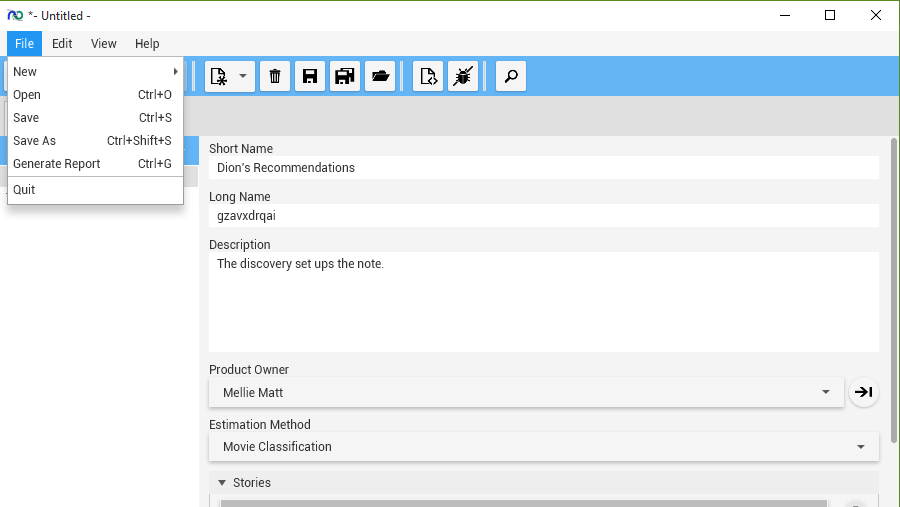
\includegraphics[width=\textwidth]{images/screenshots/file_menu.PNG}
	\caption{File menu}
	\label{fig:file_menu}
\end{figure}

When there is currently a file being viewed, its name will appear in the window title. If there are any unsaved changes, then a star will appear beside the name to indicate this. If you wish to save to a file, you may choose the "Save" option, which will overwrite the currently loaded file; or, you may choose the "Save As" option to create a new file. Example is shown in Figure~\ref{fig:file_menu}

% A guide to navigating the app
\section{Navigation}

There are various means of navigating through Murcs. The primary method is to select items from the side bar that you wish to inspect. If you wish to inspect a different item type then the choice box above the side bar may be used to inspect different elements.

\begin{figure}[H]
\centering
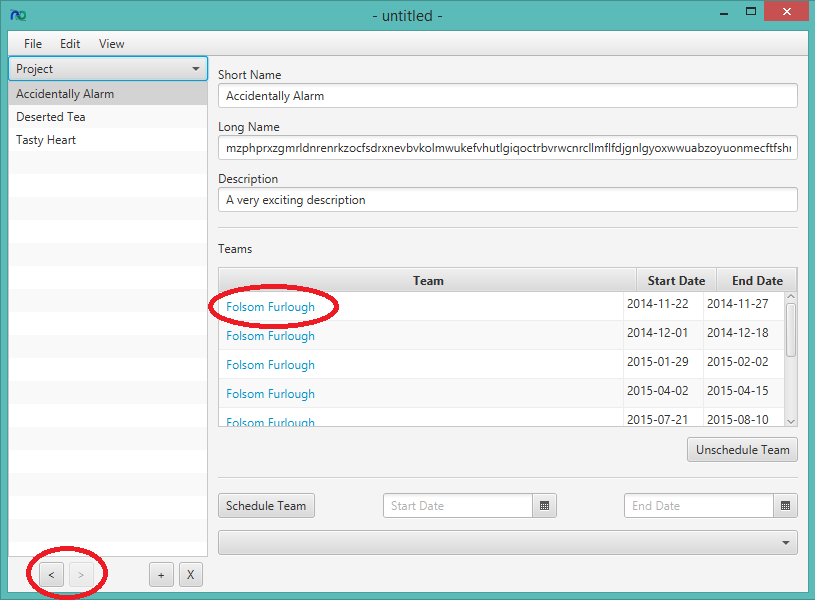
\includegraphics[width=\textwidth]{images/screenshots/navigation.PNG}
\caption{Methods of Navigation}
\label{fig:new_project}
\end{figure}

In order to conveniently go back to previously selected items, there are backward and forward buttons positioned below the side bar that take the application to the previous page. This works up to a maximum of five places. If the undo feature is used then position information will be lost.

In addition to these, when an item is mentioned within another items editor, it exists as a hyperlink to that items editor window.

It is also possible to go back and forward by holding the ALT key and pressing the LEFT and RIGHT arrow.

% A guide to using the toolbar, for the lovely end users out there
\section{Tool Bar}

There is a tool bar for performing various frequently used commands. These are listed below in their order from left to right in the given figure:

\begin{itemize}
\item Back - navigates back to the previous item
\item Forward - navigates forward to the next item
\item Revert - reverts the project back to it's original form
\item Undo - undoes the last change
\item Redo - redoes the last change
\item Add new item - you can specify the type in the drop down
\item Delete current item
\item Save the project
\item Save As
\item Open a new project
\item Generate a report - opens report generation window
\item Send feedback to the developers on bugs
\item Search the application
\end{itemize}

\begin{figure}[H]
\centering
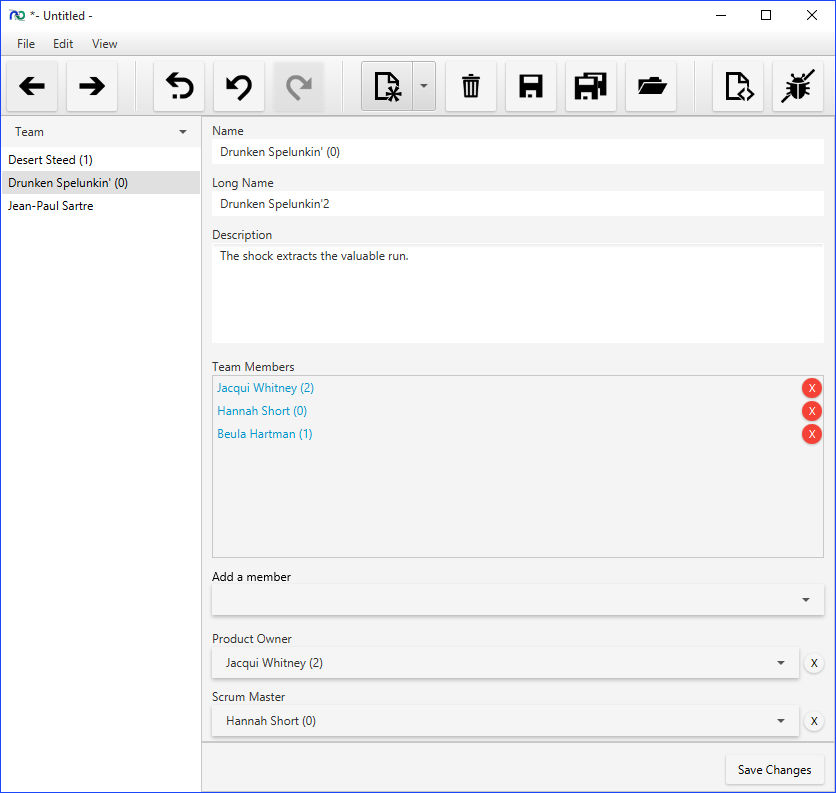
\includegraphics[width=\textwidth]{images/screenshots/toolbar.PNG}
\caption{Tool Bar}
\label{fig:new_project}
\end{figure}

It is also possible to hide sections of the toolbar. In order to do this right click on the toolbar (not on one of the buttons) and a context menu will appear with the sections of the toolbar that you can show and hide, as shown in the figure below. You can also access this within the View menu under Toolbar.

\begin{figure}[H]
\centering
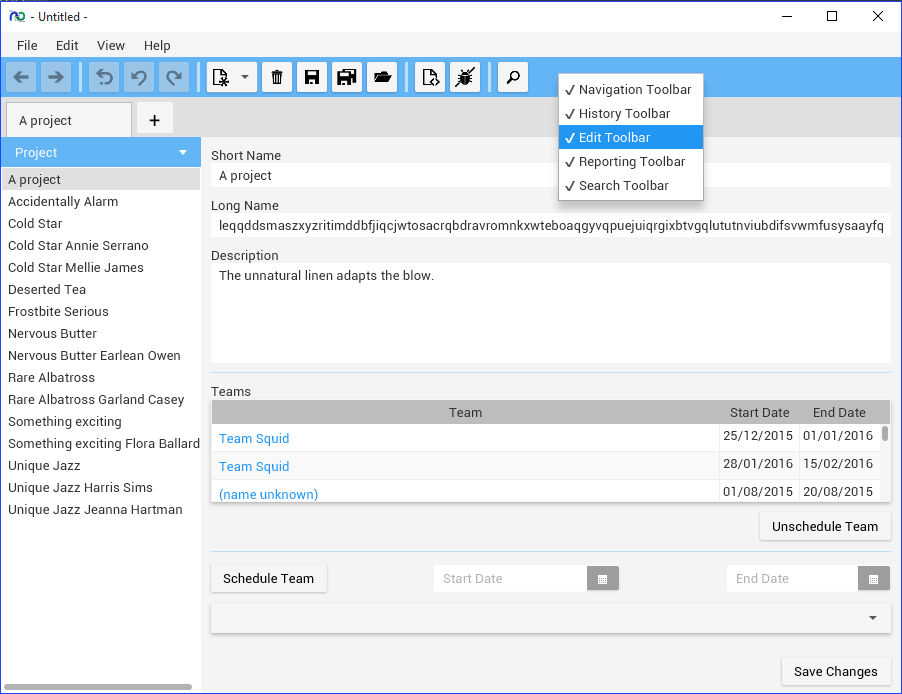
\includegraphics[width=\textwidth]{images/screenshots/toolbar1.PNG}
\caption{The Tool Bar Hides (Because you're scary)}
\label{fig:new_project}
\end{figure}

% A guide for managing person
\section{People Maintenance}

Managing People
\newline\newline
People can be easily added to Murcs and then used as necessary. 
\newline
Creating new people is very simple. There are two ways of doing it, the first is to make sure you have the People selected in the display list as shown below. Then click the new button on the toolbar.

\begin{figure}[H]
\centering
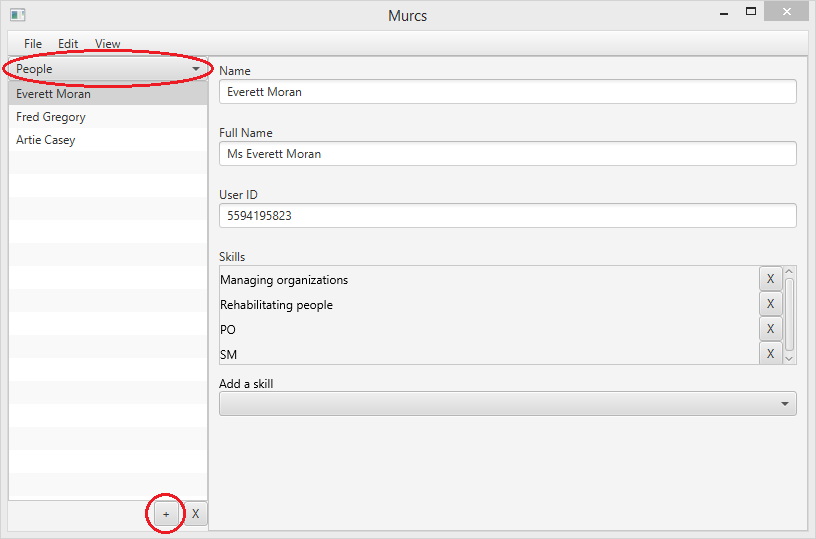
\includegraphics[width=\textwidth]{images/screenshots/people1.PNG}
\caption{Adding a Person Method 1}
\label{fig:new_project}
\end{figure}

The other method is to select File/New/Person from the File menu at the top of the application as shown in the fig below.

\begin{figure}[H]
\centering
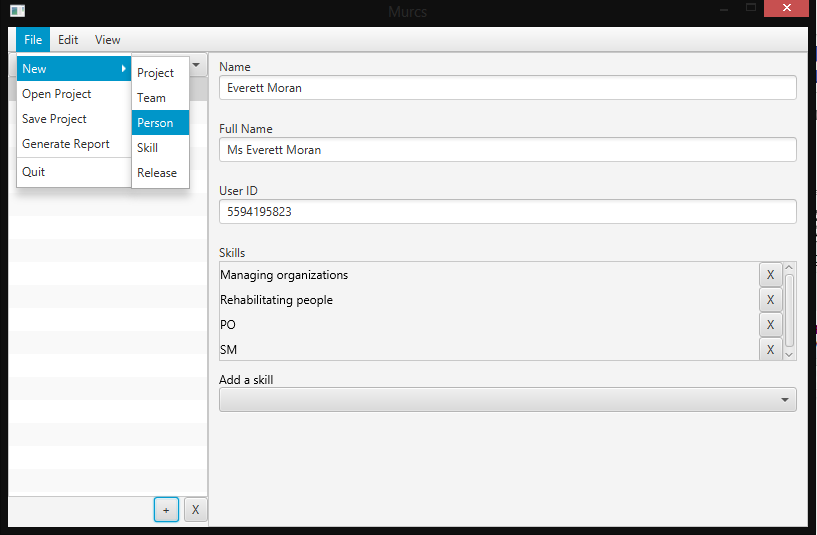
\includegraphics[width=\textwidth]{images/screenshots/people4.PNG}
\caption{Adding a Person Method 2}
\label{fig:new_project}
\end{figure}

Once you have clicked the add button or selected file/new/person a dialog will appear that asks for information about the new person you are creating. The minimum requirements for this are the Name and UserID, all of the other fields are optional. These fields include, a full name and a method for adding skills to the person.

\begin{figure}[H]
\centering
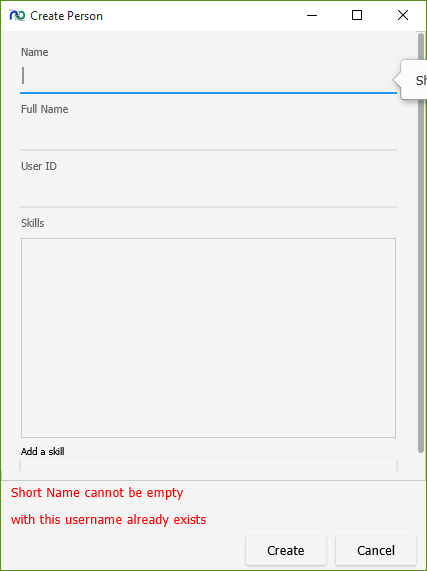
\includegraphics[width=\textwidth]{images/screenshots/people2.PNG}
\caption{Person Creation Dialog}
\label{fig:new_project}
\end{figure}

To add a skill simply select it from the drop down list (this is populated based on the skills you have added already) and it will appear in the list of skills. Then to remove a skill simply click x next to the skill. Note: If you add the PO skill to a person and then assign them to be PO of a Team and then remove the PO skill from them then they will be removed from the position of PO on that team.

\begin{figure}[H]
\centering
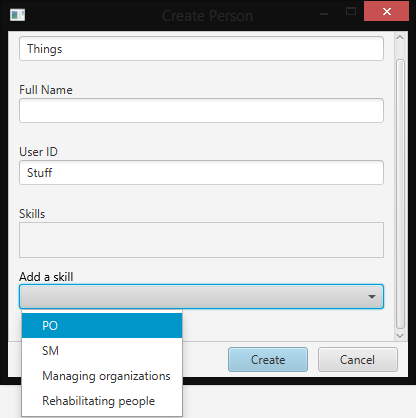
\includegraphics[width=\textwidth]{images/screenshots/people3.PNG}
\caption{Person adding/removing Skills}
\label{fig:new_project}
\end{figure}

In order to delete a person simply select it from the side list and click the X button next to the add button in the list display. When a person is deleted it will be removed from any place it is referenced in the application.

Once you have a person created you can add them to Teams which is covered in the Teams section of this user guide.

% A guide for managing teams
\section{Team Maintenance}

Managing Teams
\newline\newline
In murcs teams are groups of people who will work together on certain projects. The team will include information such as the short and long name of the team, a list of all the members in the team and the ability to add and remove members and a method of setting the product owner and scrum master of the project.
\newline
Firstly in order to create a team there are two methods, very similar to people, you either select Teams in the display list and then press the plus button or you select File/New/Team. Both of these methods will open up a create team dialog as displayed below.

\begin{figure}[H]
\centering
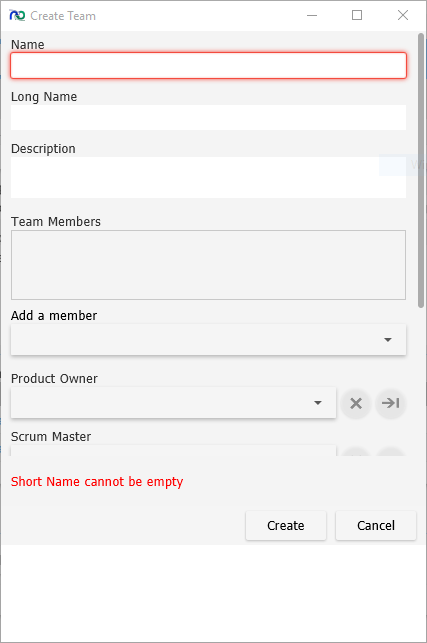
\includegraphics[width=\textwidth]{images/screenshots/teams1.PNG}
\caption{Creating a Team}
\label{fig:new_project}
\end{figure}

Once this has appeared you need to enter a name for the team, this is the only compulsory field. The other fields can be filled in and to add team members simply select from the drop down box of members in the add team member drop down box, as shown below. After selecting someone they will appear in the Team Members area and to then remove them simply click the X box next to the person.

\begin{figure}[H]
\centering
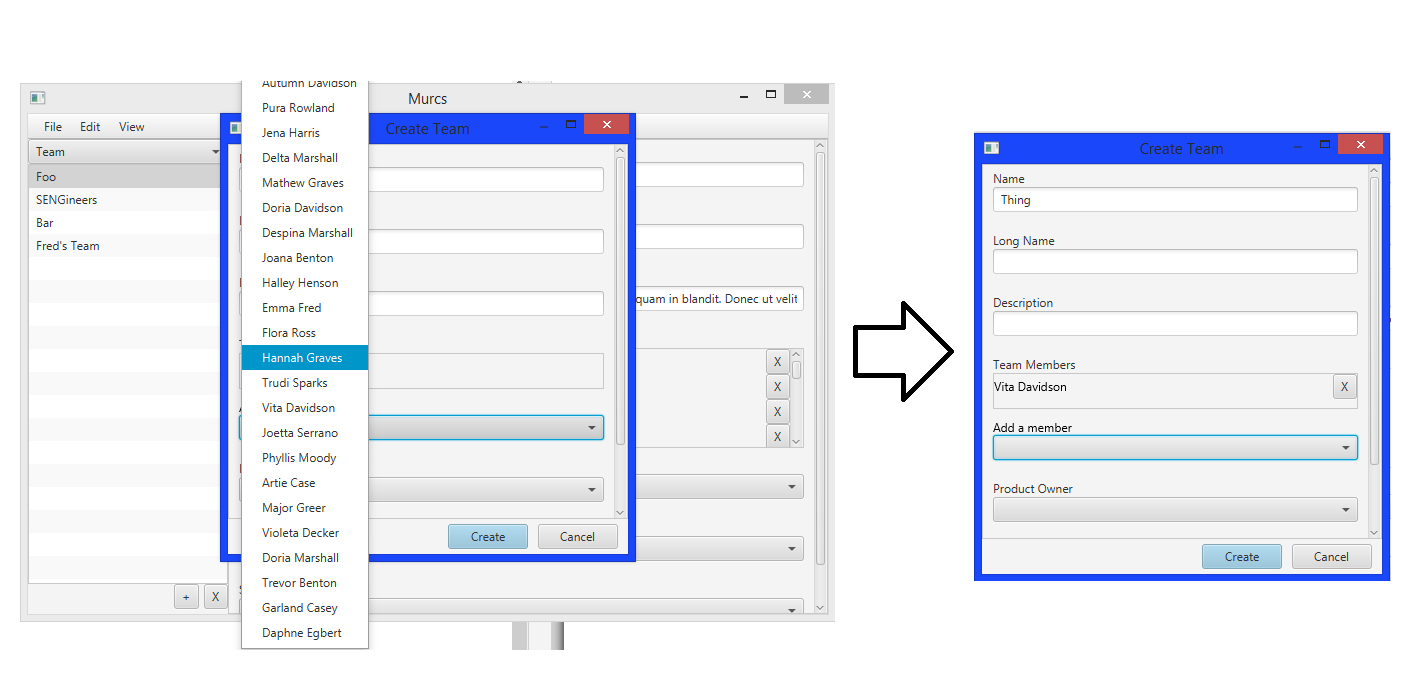
\includegraphics[width=\textwidth]{images/screenshots/teams2.PNG}
\caption{Adding People to a Team}
\label{fig:new_project}
\end{figure}

Once you finished editing the values you want simply press the create button. If there are any problems creating the team (usually if you haven't filled in a necessary field) then the team will not be created and you will get an error message at the bottom of the creation window as shown below.

\begin{figure}[H]
\centering
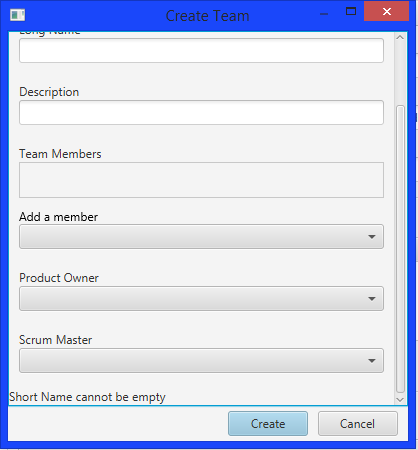
\includegraphics[width=\textwidth]{images/screenshots/teams3.PNG}
\caption{Error Creating a Team}
\label{fig:new_project}
\end{figure}

When you have created your team you can edit it by selecting the team section from display list and then clicking on the team you want to edit, as shown below. The edit form works in exactly the same way as the create form.

\begin{figure}[H]
\centering
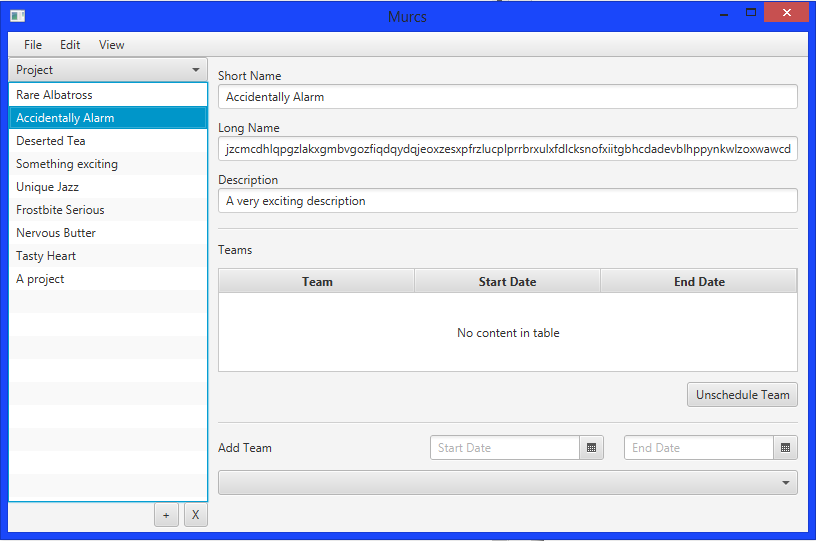
\includegraphics[width=\textwidth]{images/screenshots/teams4.PNG}
\caption{Editing a Team}
\label{fig:new_project}
\end{figure}

If at some stage you wish to delete a team then simply select it in the display list and click the X button and it will show a dialog confirming you want to delete and all the places that the team is used. If you choose to delete it then it will be deleted and removed from any of the places it is linked to other items (for instance all the people in it will become unassigned again).

\begin{figure}[H]
\centering
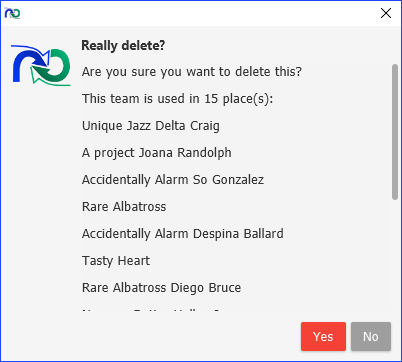
\includegraphics[width=\textwidth]{images/screenshots/teams5.PNG}
\caption{Deleting a Team}
\label{fig:new_project}
\end{figure}

For teams you can also view the number of peer programming hours and people have done within the team. If you want to see this simply go to the peer programming pane of the team editor and it will show you a list of all of the pairs of people who have worked together on every sprint the team has worked on, as shown in the figure below.

\begin{figure}[H]
\centering
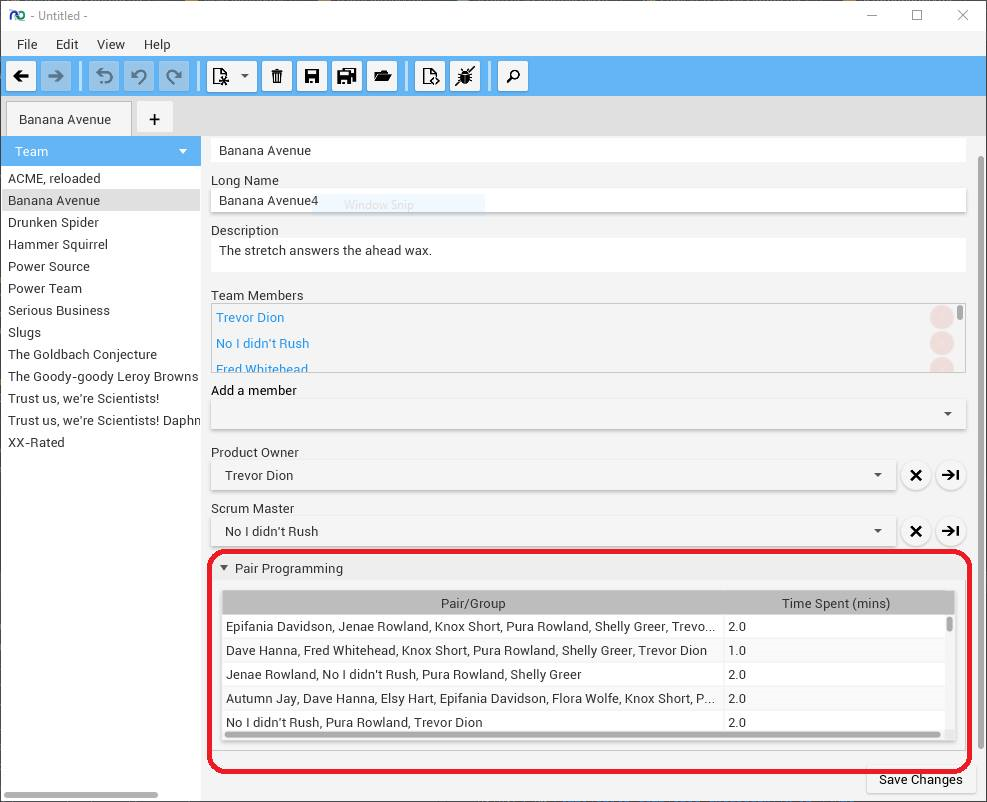
\includegraphics[width=\textwidth]{images/screenshots/teams6.PNG}
\caption{Viewing Peer Programming}
\label{fig:new_project}
\end{figure}


% A guide for managing projects
\section{Project Maintenance}

Managing Projects
\newline\newline
One of the main purposes of murcS is to manage Projects. Projects are exactly what they sound like, they're projects. You can currently change the name of the project, it's description, add allocations for when you want a team to be working on that particular project and you can also link Projects to releases which is when you want to make a release for a certain project.
\newline
When you wish to create a new project similarly to everything else, simply select project from the display list and click the add bottom at the bottom of list or select File/New/Project from the file menu. When you've done this a creation dialog will appear as shown below.

\begin{figure}[H]
\centering
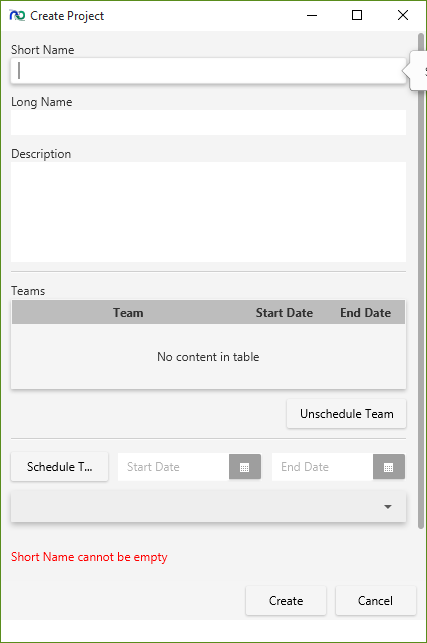
\includegraphics[width=\textwidth]{images/screenshots/projects1.PNG}
\caption{Creating a Project}
\label{fig:new_project}
\end{figure}

Within this dialog the only compulsory field is the project short name (which is what it will be displayed as in the display list), all fields can be edited later on so there is no need to fully fill this out when you create it.
\newline
The other fields that you can edit in here include the long name of the project, it's description and finally the scheduling system for assigning teams to work on the project over certain periods in time. To assign a team to a project simply select the team you want to assign from the drop down box of teams and then add a start and end date (these dates must makes sense - end comes after start) and then the team will appear in the assigned teams table as shown below.

\begin{figure}[H]
\centering
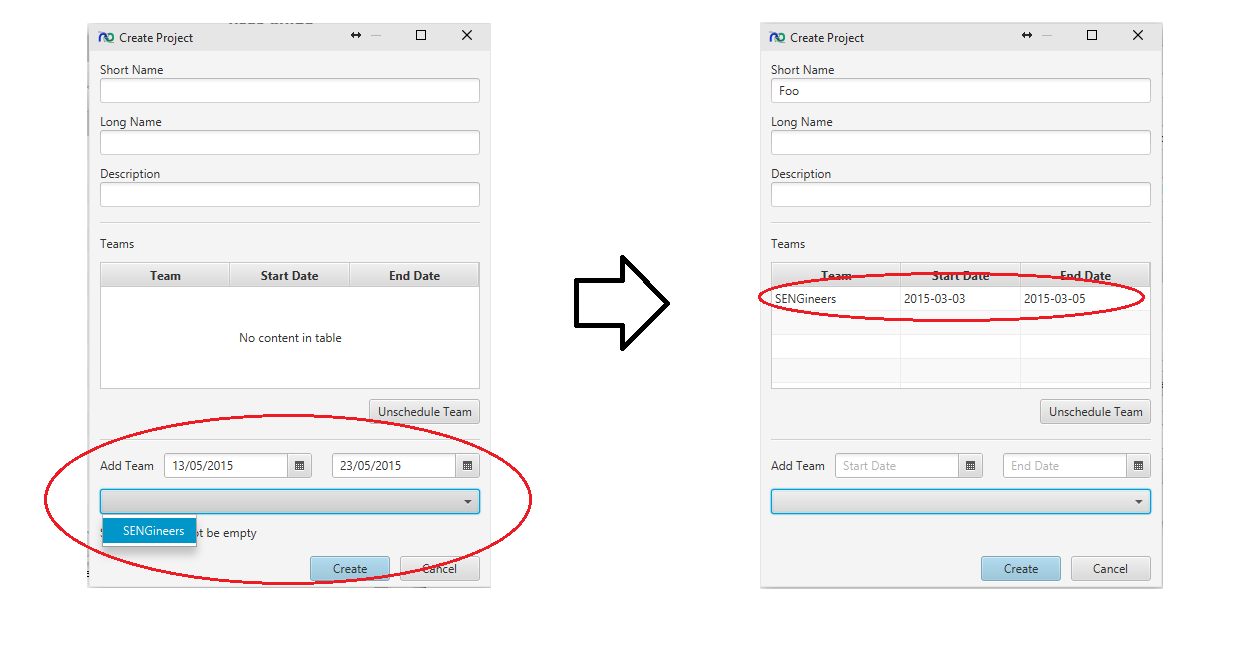
\includegraphics[width=\textwidth]{images/screenshots/projects2.PNG}
\caption{Scheduling a Team to a Project}
\label{fig:new_project}
\end{figure}

If you ever want to remove a team that has been assigned to the project you can do so by selecting it in the list of assigned teams and then click the Unschedule Team button and the team will be unscheduled, as shown below.

\begin{figure}[H]
\centering
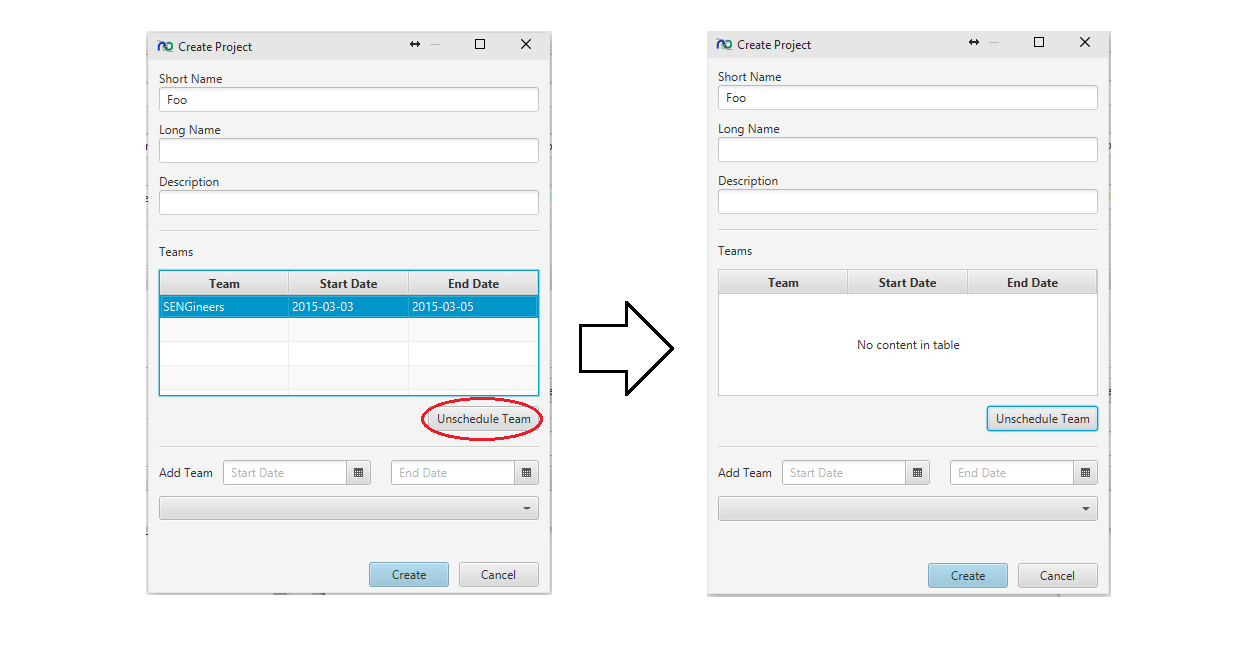
\includegraphics[width=\textwidth]{images/screenshots/projects3.PNG}
\caption{Unscheduling a Team from a Project}
\label{fig:new_project}
\end{figure}

Once you've created your project you can easily edit it in exactly the same format that you created it by selecting it from the display list, similarly to people, releases, teams etc. If you ever want to delete a project you can do this in a very similar way to deleting other items. You will get a warning before deleting it as with all the other objects, however with this warning if you delete the project all associated releases will also be deleted as well as they are no longer linked to project and are therefore pointless.

% A guide for managing skills
\section{Skill Maintenance}

Managing Skills
\newline\newline
Within Murcs it is very easy to manage skills. The main purpose is to give an idea of what individual people are experienced in. Skills should be generic so that they can be added to multiple people. Some examples might be C\#, Java, Python, Talking.
\newline
When you wish to create a new skills simply go to the display list and select skills. Then following the same process as People, Teams etc. either click the add button in the bottom of the list or select File/New/Skill. Once you have done this a creation dialog will appear as shown below.

\begin{figure}[H]
\centering
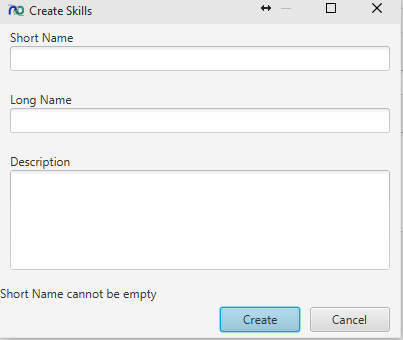
\includegraphics[width=\textwidth]{images/screenshots/skills1.PNG}
\caption{Creating a Skill}
\label{fig:new_project}
\end{figure}

When you create a skill the only compulsory field is the short name, this should be along the lines of C\# or Java. The long name is optional and could be for example C Sharp. The description should just detail what the skill means in particular.
\newline\newline
When you've created a skill you can then edit them and delete them in a very similar way to teams and people. Simply select the skill you want to edit or delete and then either edit it in the edit pane that appears in the main screen or click the delete button at the bottom of the display list. If you are deleting the skill it will tell you where the skill is used and if you still want to delete the skill it will delete it from all of the people it was linked with. The only skills that are not deletable are PO and SM as theses are necessary for Scrum.

% A guide for managing releases
\section{Release Maintainence}

Managing Releases
\newline
Releases for a project can easily be added, deleted and updated using murcS. To begin select 'Releases' in the Display Choice picker (circled below)

\begin{figure}[H]
\centering
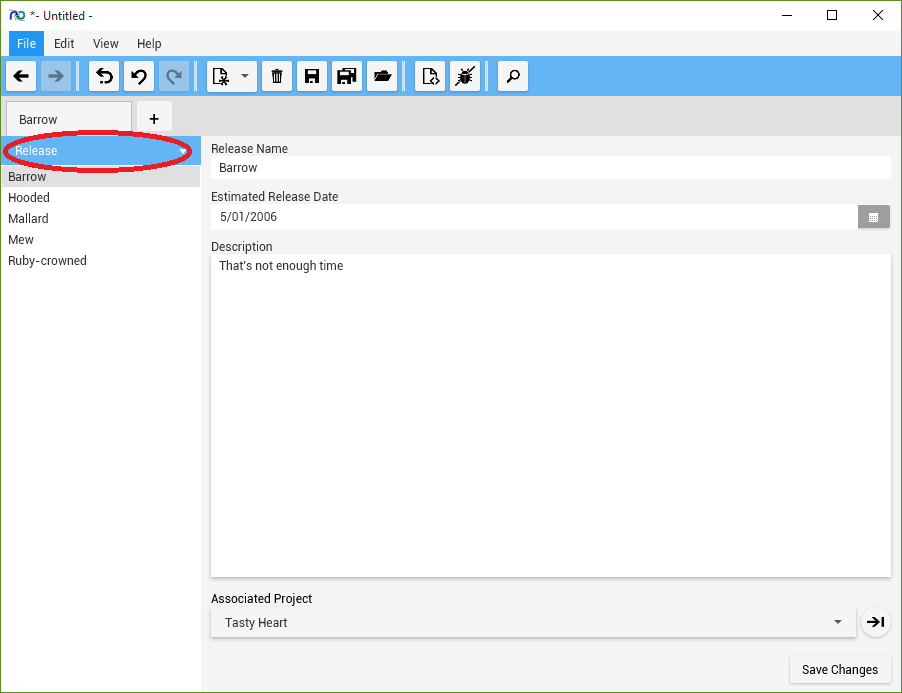
\includegraphics[width=\textwidth]{images/screenshots/releases1.PNG}
\caption{The Display Choice Picker}
\label{fig:new_project}
\end{figure}

Creating Releases
\newline
Now, to add a new release, simply press new button (circled below) on the toolbar and you will be presented with a form for creating a new release. Note that new button is context sensitive and the type of element you create will depend on what section of the application you are in.

\begin{figure}[H]
\centering
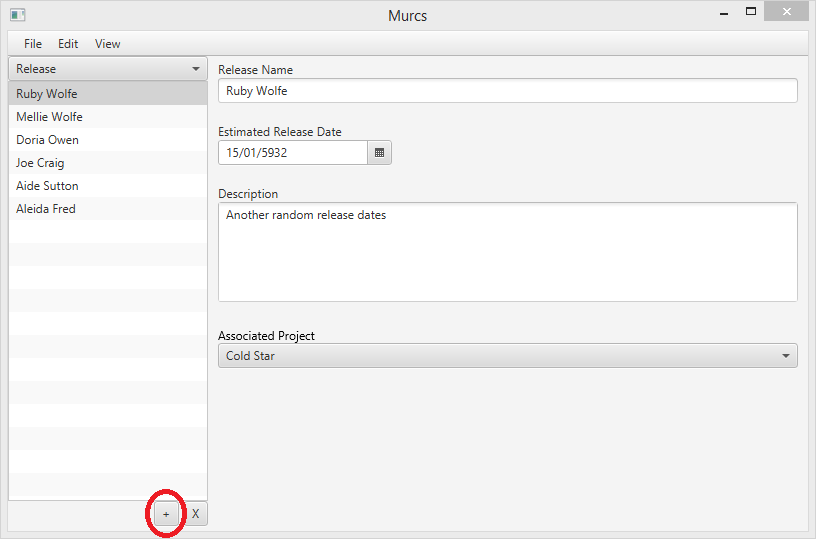
\includegraphics[width=\textwidth]{images/screenshots/releases2.PNG}
\caption{The Add Button}
\label{fig:new_project}
\end{figure}

You will then be presented with a form for creating a new release which should look something like the one shown here:

\begin{figure}[H]
\centering
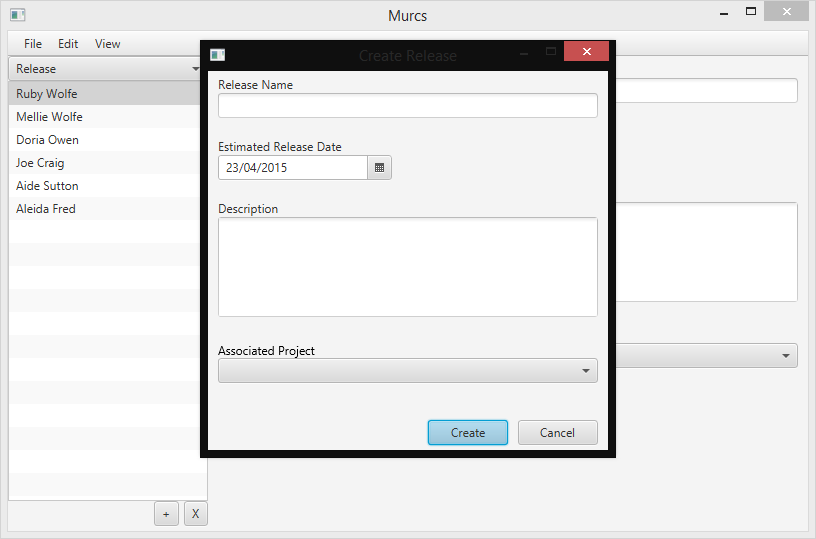
\includegraphics[width=\textwidth]{images/screenshots/releases3.PNG}
\caption{Creating a new release}
\label{fig:new_project}
\end{figure}

Constraints
\newline
There are several constraints you need to take into account when creating a release. Firstly, a release must be given a unique name within the platform, so it can quickly and easily be identified within the application. If a constraint is not met then a small message will be shown explaining the problem.

Editing Releases
\newline
Any release can be edited by selecting it from the Display List. Upon selection, the form on the right will be populated with all the fields that you can edit. Any changes you make will be automatically saved.

\begin{figure}[H]
\centering
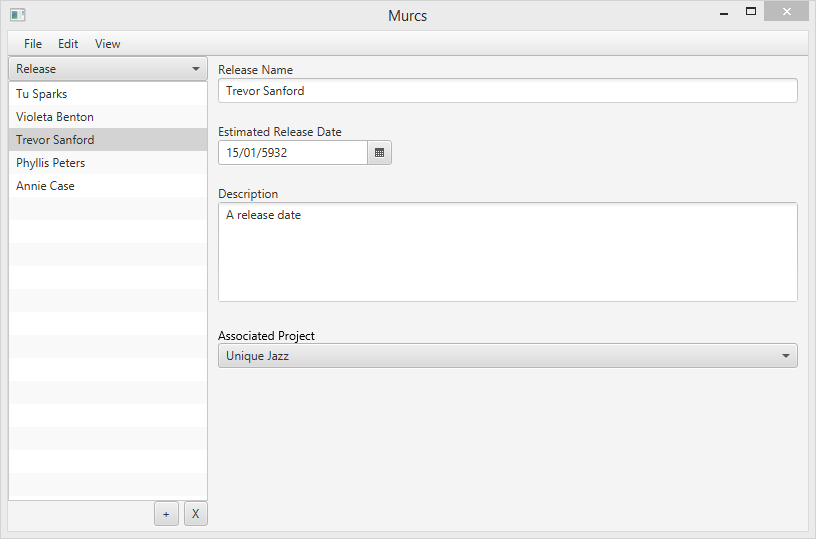
\includegraphics[width=\textwidth]{images/screenshots/releases4.PNG}
\caption{Editing the Release Named 'Barrow'}
\label{fig:new_project}
\end{figure}

Deleting Releases
\newline
Releases can be deleted in the same manner as any other element, by clicking the delete button on the toolbar. For a more in depth explanation, see the element deletion section of this guide


% A guide to maintaining stories
\section{Story Maintenance}

Managing Stories
\newline
Stories for a project can easily be added, deleted and updated using Murcs. To begin select 'Story' in the Display Choice picker (circled below)

\begin{figure}[H]
\centering
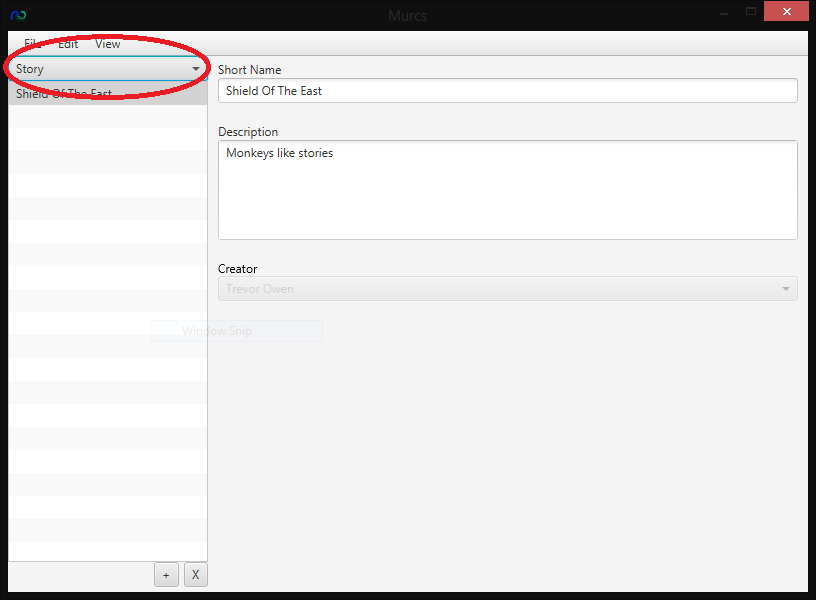
\includegraphics[width=\textwidth]{images/screenshots/stories1.PNG}
\caption{The Display Choice Picker}
\label{fig:new_project}
\end{figure}

Creating Stories
Stories can be created in two different ways, by clicking the add button on the toolbar or by navigating File->New->Story.

\begin{figure}[H]
\centering
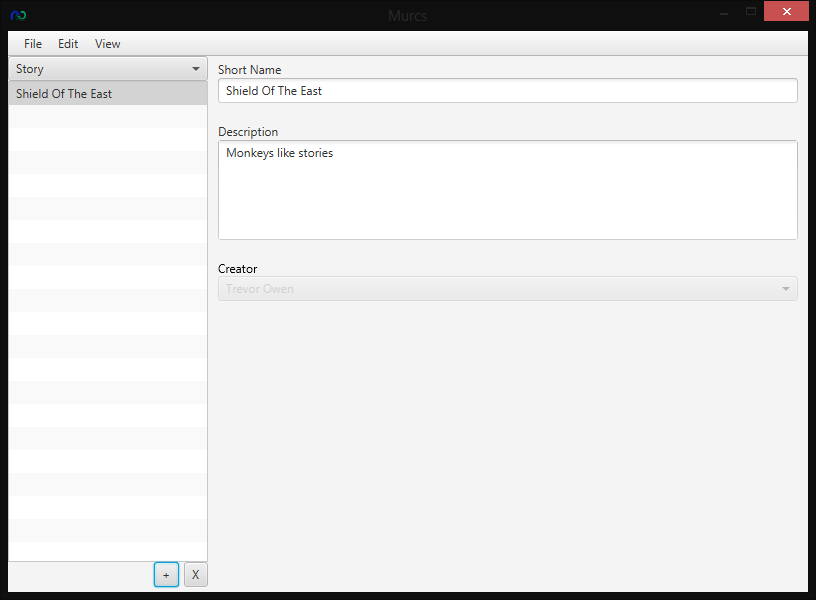
\includegraphics[width=\textwidth]{images/screenshots/stories2.PNG}
\caption{The Story Creation Dialog}
\label{fig:new_project}
\end{figure}

Whichever way you chose to create your story you will have been greeted with the following 'Story Creation Dialog' (pictured below). When creating a story you can specify a number of different fields. 

Name:
This is the name of your story. It must not be empty and must be unique, but you can change it later. This will show up in the display list, so make it recognizable!

Description:
To make life easier for your team it is helpful to know what a story is about. This is where the description field comes in. The description can be anything you like, but is most useful if it describes the story. You can change the description at any point.

Creator:
This field stores the original creator of the story. It cannot be changed after the project has been created, so make sure you get it right first time.

Updating:
To update an existing story, simply select it from the display list. In the below picture we are editing the story known as 'A Story.' Note how the creator field is greyed out and cannot be changed.

\begin{figure}[H]
\centering
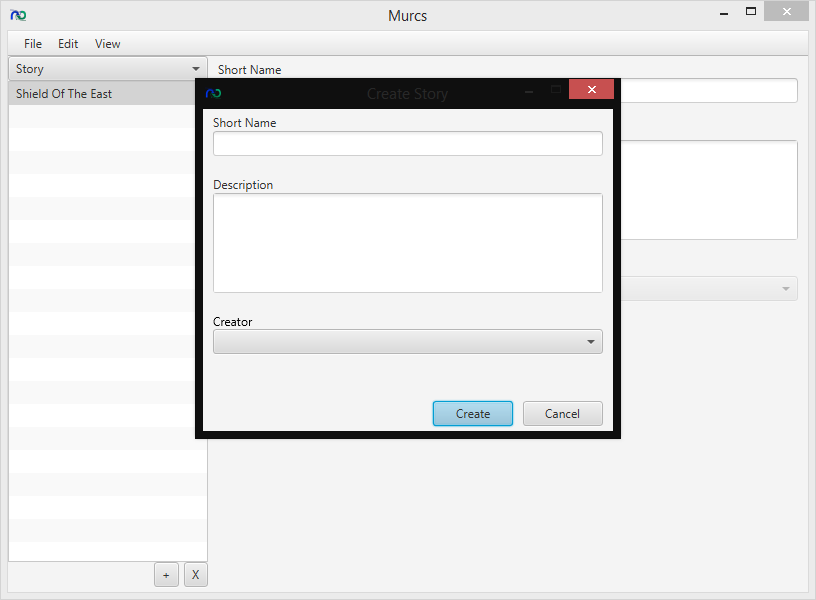
\includegraphics[width=\textwidth]{images/screenshots/stories3.PNG}
\caption{The Editing Pane}
\label{fig:new_project}
\end{figure}

Story State\newline
The Story State property (circled below) defines the state a story is currently in. If you try to change this but the state is not supported an error message will be displayed at the bottom of the editor. \newline

Requirements\newline
None: No requirements\newline
Ready: Story is in a backlog, story has at least one AC and story is estimated

\begin{figure}[H]
\centering
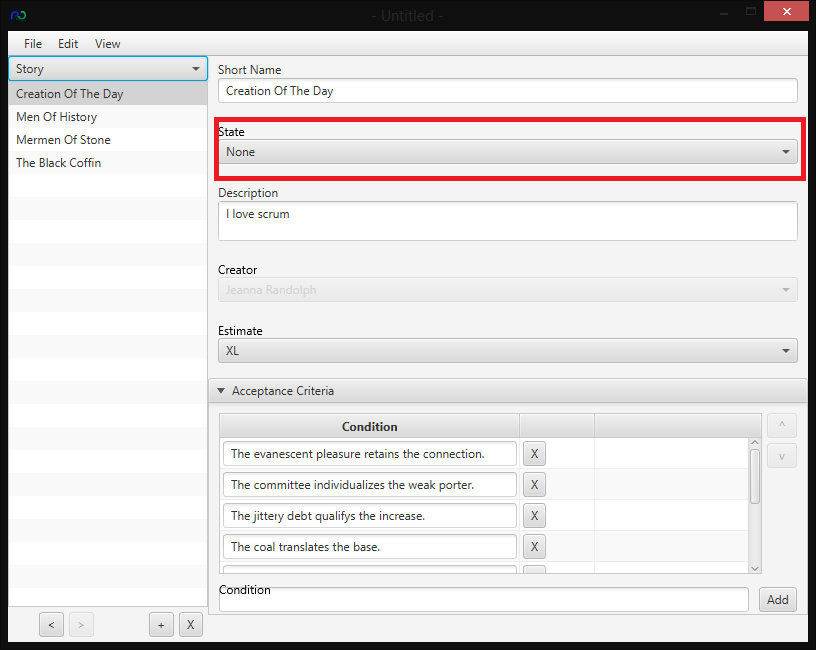
\includegraphics[width=\textwidth]{images/screenshots/Readiness1.PNG}
\caption{The Story State Property}
\label{fig:new_project}
\end{figure}

Estimating\newline
To create an estimate for a story, your story must first be part of a backlog and have at least one Acceptance Condition (see below). The scale you estimate on depends on the scale specified in the backlog that this story is attached to. If you change this type on the backlog the program will do it's best to work out what the equivalent is on the new scale.

\begin{figure}[H]
\centering
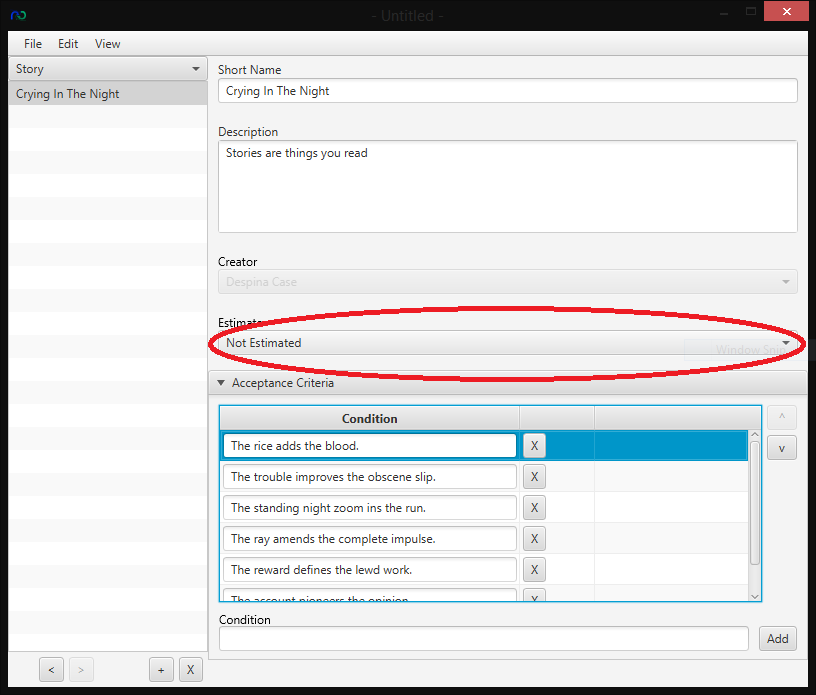
\includegraphics[width=\textwidth]{images/screenshots/Estimate1.PNG}
\caption{The Estimate Property}
\label{fig:new_project}
\end{figure}

Acceptance Criteria (ACs)\newline
A story can have any number of acceptance criteria. However, you should note that there are some things you cannot do to a story if it does not have an ACs (such as estimating that story or changing its state to ready). Acceptance criteria can be managed using "Acceptance Criteria" pane (marked below) while editing a story.

\begin{figure}[H]
\centering
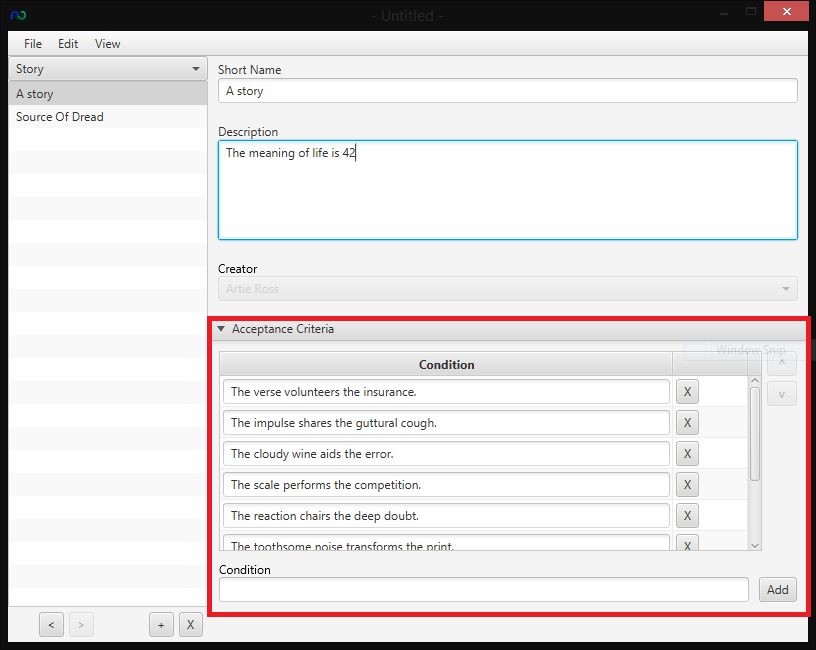
\includegraphics[width=\textwidth]{images/screenshots/AcceptanceCriteria1.PNG}
\caption{The Acceptance Criteria Pane}
\label{fig:new_project}
\end{figure}

You can create a new Acceptance Condition by typing in the "Add Condition" text field (marked below) and pressing the add button. New acceptance conditions will be added at the end of the list by default.

\begin{figure}[H]
\centering
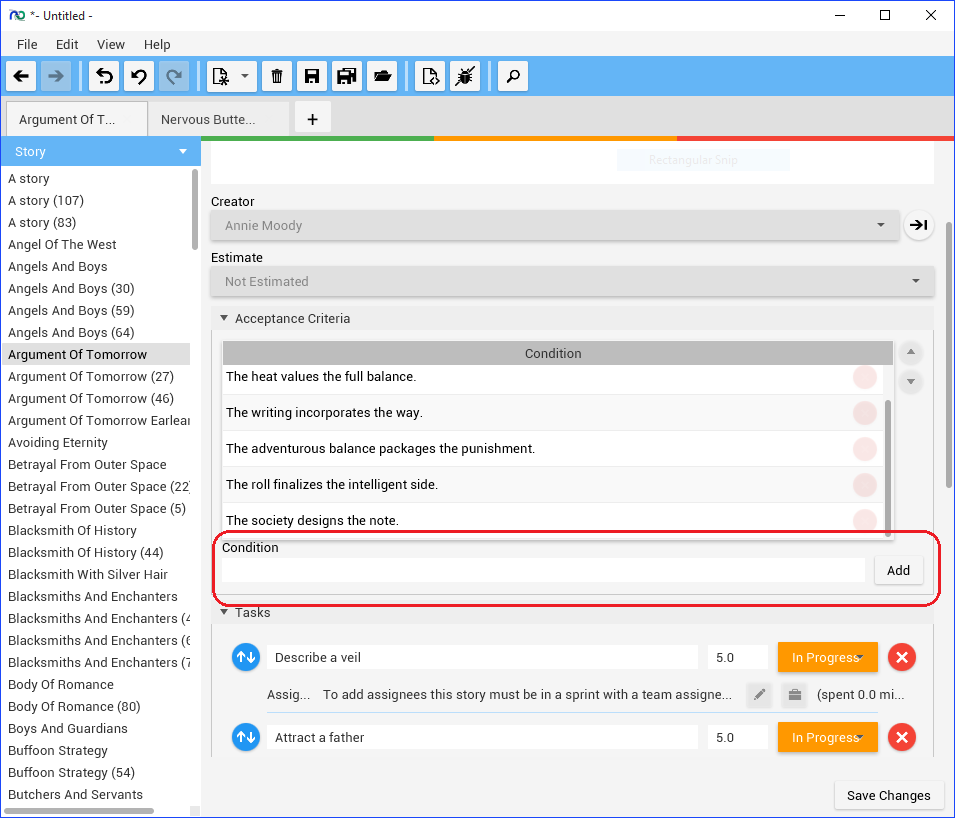
\includegraphics[width=\textwidth]{images/screenshots/AcceptanceCriteria2.PNG}
\caption{The Add Condition Field}
\label{fig:new_project}
\end{figure}

You can edit the condition on an AC by simply typing in the relevant text field. Your changes will be saved automatically, when you click away. Similarly, you can delete a condition using the 'X' button in the second column of the table.
\newline\newline

Acceptance Conditions can also be moved up and down in the list, depending on their priority. To do this, use the up and down arrows (marked below). A condition cannot be moved up from the top of the list or down from the bottom.

\begin{figure}[H]
\centering
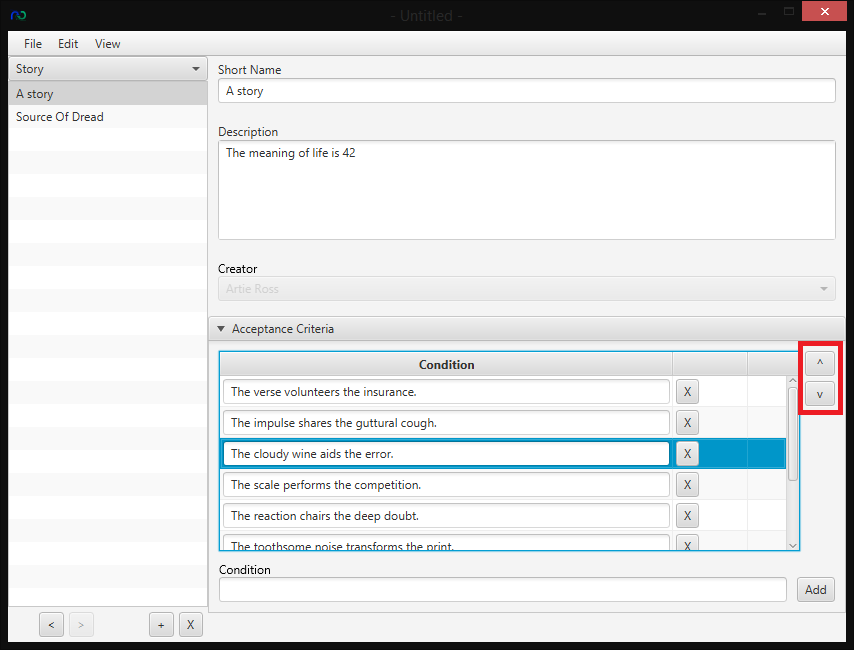
\includegraphics[width=\textwidth]{images/screenshots/AcceptanceCriteria3.PNG}
\caption{The Priority Buttons}
\label{fig:new_project}
\end{figure}

Dependencies\newline
You can manage dependencies in the dependencies area of the story pane. To add a story as a dependency, simply start typing its name or select it from the list box provided. Dependencies must be transitive (they cannot cause dependency cycles). Attempting to add a dependency that will cause a cycle will result in an error.\newline
Removing a dependency is done in the same way as for Acceptance Criteria. Pressing the 'X' button on the right hand side of each dependency will remove it from the story.\newline
Depth of a dependency, as indicated to the left side of the 'X' button, describes the maximum number of dependencies that the dependency itself transitively depends on.\newline\newline

Deletion\newline
To delete a story, simply press the delete button (the bin in the tooblar). You will be greeted with a confirmation dialog that will notify you of all the places the story is used. From this dialog you can go through with the deletion or cancel if you change your mind. For more information, see the 'Element Deletion' section of this guide.

\begin{figure}[H]
\centering
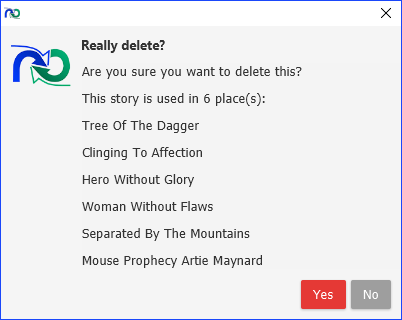
\includegraphics[width=\textwidth]{images/screenshots/stories5.PNG}
\caption{Deleting a Story}
\label{fig:new_project}
\end{figure}

% A guide to maintaining tasks
\section{Task Maintenance}

Managing Tasks
\newline
Tasks can be created and added to a story from within the story editor. To begin, expand the task section.

\begin{figure}[H]
\centering
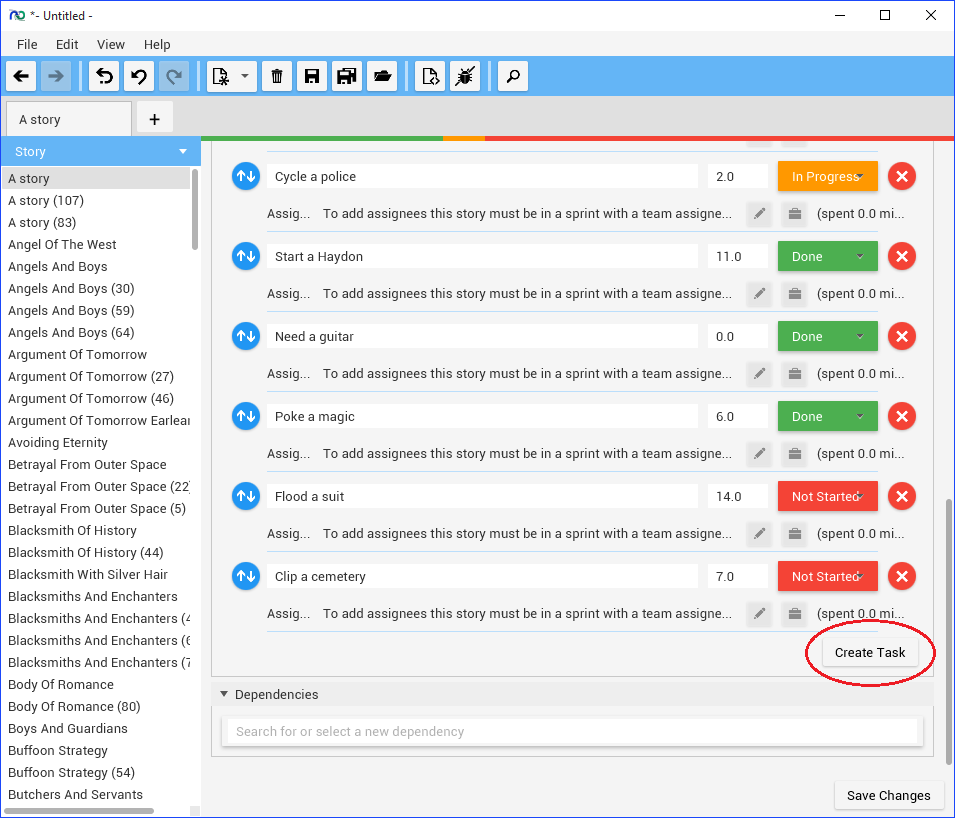
\includegraphics[width=\textwidth]{images/screenshots/task_1.png}
\caption{Create a new task}
\label{fig:new_project}
\end{figure}

Click on the "Create Task" button, circled in red. It will add a new blank task for you to fill the details in for.

\begin{figure}[H]
\centering
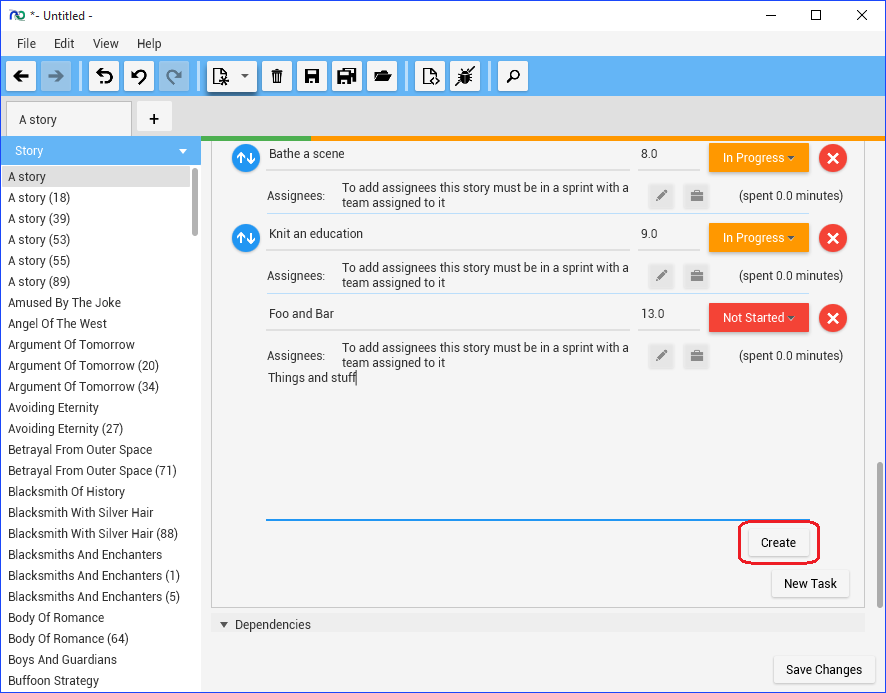
\includegraphics[width=\textwidth]{images/screenshots/task_2.png}
\caption{Save the newly created task}
\label{fig:new_project}
\end{figure}

Once the name and estimate fields have valid values entered, you will be able to click on the "Create" button and save the task to that story. Now, it will always be there when you come back to that story.

\newline

Note:
\newline
You can not make two tasks with the same name.

% A guide to backlog maintenance
\section{Backlog Maintenance}

Managing Backlogs
\newline\newline
Backlogs can be easily maintained. Creating a backlog is the exact same process as creating any other type of model (via the File menu or the new button on the toolbar). Once you have opened the create window the only two things necessary for the creation of a backlog are the short name and the PO assigned to the backlog.
\newline
Adding a new story to a backlog is easy. Simply select it from the story drop down (optionally give it a priority) and then press add. Prioritised stories will appear at the top of the table, ordered by their priority. Unprioritised stories will appear below them in alphabetical order. To remove a story simply click the X next to it.

\begin{figure}[H]
\centering
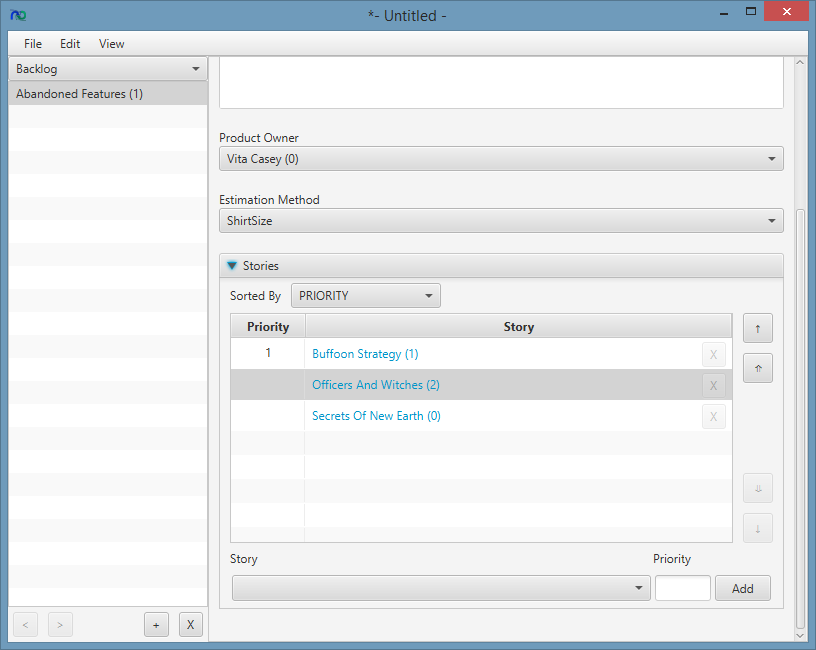
\includegraphics[width=\textwidth]{images/screenshots/backlogs.PNG}
\caption{The Backlogs Edit Pane}
\label{fig:new_project}
\end{figure}

\bigskip
To change the priority of a story simply select it and click on the up and down arrows to the side of the table; the small arrow buttons shift the story by one priority and the large up/down arrow buttons set the story's priority to one/unprioritised respectively. Alternatively, you may specify the exact priority you wish to change a story to by clicking in the priority column for the story you wish to move, the typing the new priority and pressing enter or else just clicking away.

\begin{figure}[H]
\centering
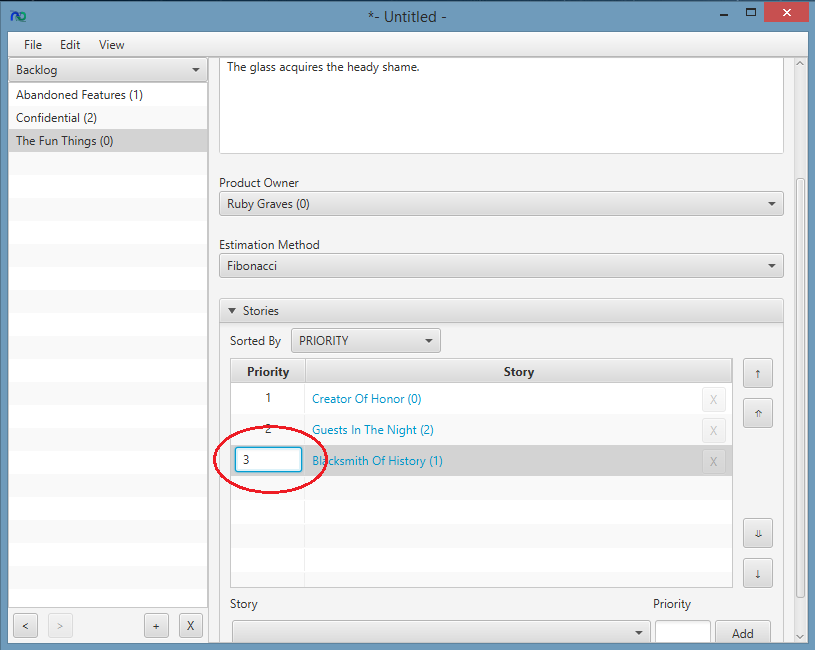
\includegraphics[width=\textwidth]{images/screenshots/editable_priority.PNG}
\caption{Editable Priorities}
\label{fig:new_project}
\end{figure}

\bigskip
If you wish to see a visual representation of the state of the backlog, you may selected the "highlight stories" item in the View menu. This will add a bar to the left of the table of stories that is coloured depending on the readiness state of the story it is beside. It is coloured red when the story depends on another story with a lower priority than itself, green when the story is ready and orange when it is almost ready but still requires an estimation.

\begin{figure}[H]
\centering
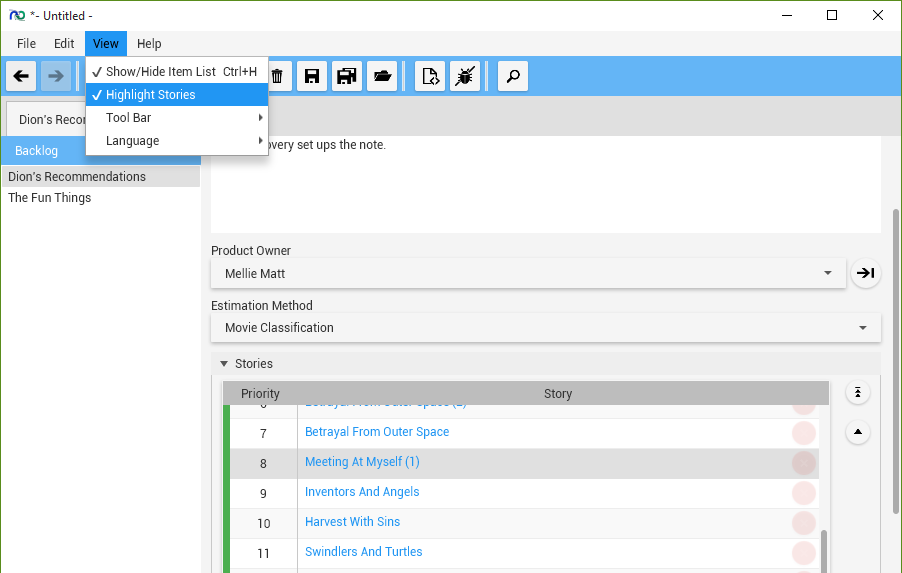
\includegraphics[width=\textwidth]{images/screenshots/story_highlighting.PNG}
\caption{Highlighting Stories}
\label{fig:new_project}
\end{figure}

\bigskip
Estimation Methods
\newline
Changing the estimation method changes how you estimate the difficulty of stories within the backlog. The supported types are Fibonacci (1,2,3,5,8,13), ShirtSizes (XS,S,M,L,XL,XXXL) and Movie Ratings (PG,G,M,R16,R18,Banned). You can change this at any time and the program will do its best to convert to the new scale. 

It is also possible to set the estimate as Not Estimated, 0 or Infinite.

\pagebreak
Estimation Workspace
\newline
The estimate workspace is a visual representation of stories in a backlog that have been grouped by common estimates. It enables the user to change the estimate of individual stories by dragging them between different estimate groups.

\begin{figure}[H]
\centering
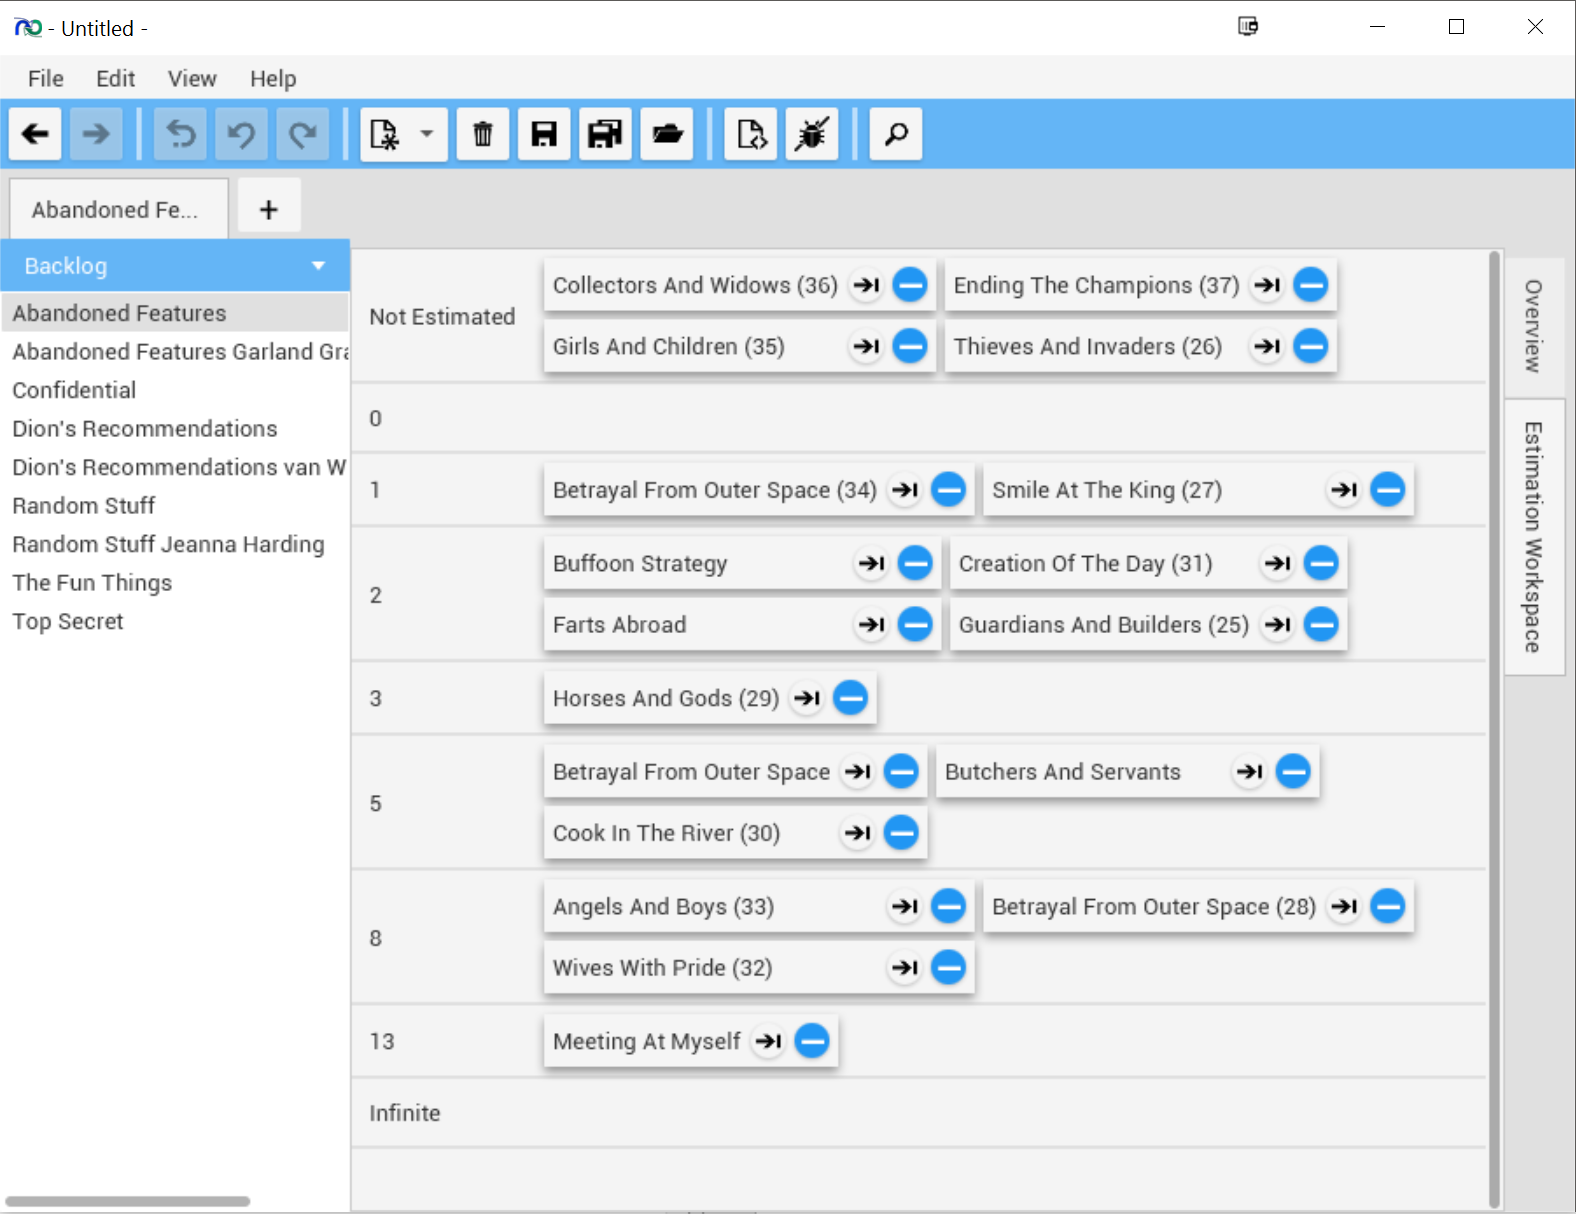
\includegraphics[width=\textwidth]{images/screenshots/estimationWorkspace1.PNG}
\caption{Estimate Workspace}
\label{fig:new_project}
\end{figure}

\pagebreak
Removing and Adding stories to the workspace:
Stories can be added or removed from the workspace via the table of stories in the backlog overview. This is in order to make it less cluttered, or if you don't want to estimate certain stories next (maybe you want to defer the story to a future sprint).
The buttons to do this are shown in the red circles

\begin{figure}[H]
\centering
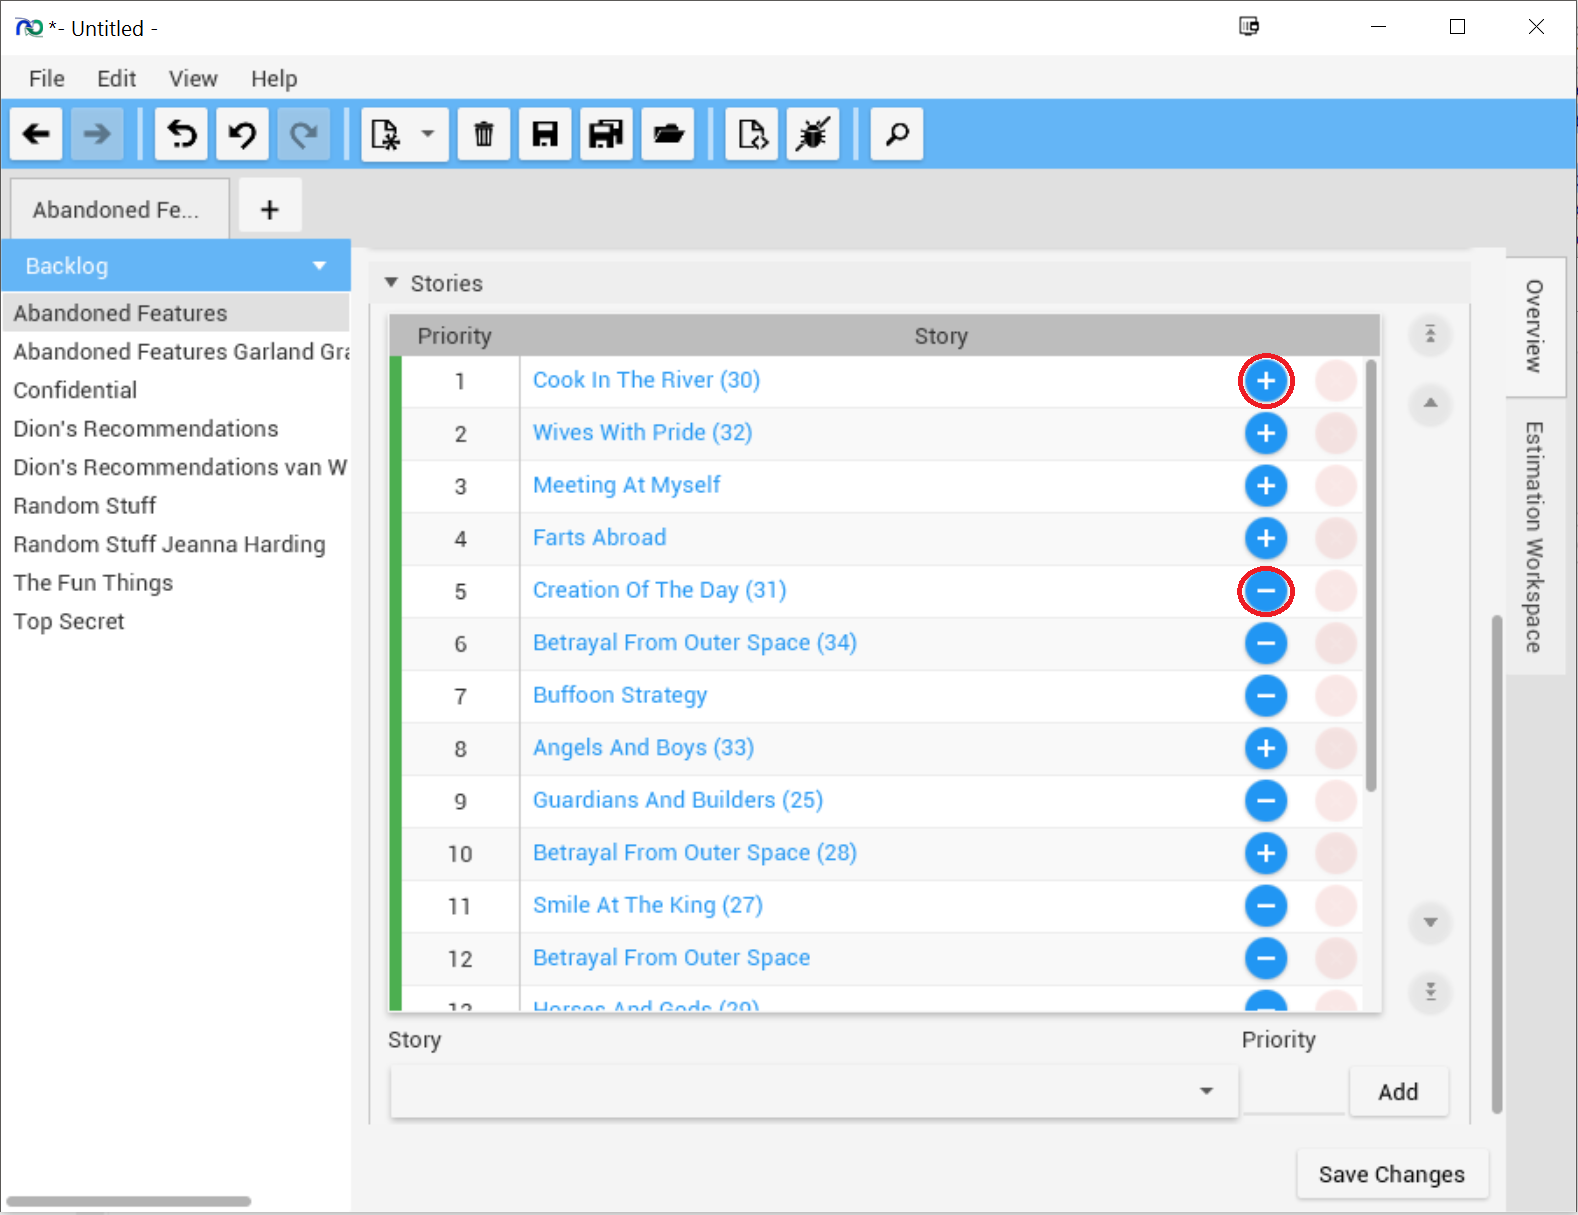
\includegraphics[width=\textwidth]{images/screenshots/estimationWorkspace2.PNG}
\caption{Adding and removing stories from the estimation workspace}
\label{fig:new_project}
\end{figure}

\pagebreak
You can also remove stories directly from the workspace by pressing the button shown in the red circle below.

\begin{figure}[H]
\centering
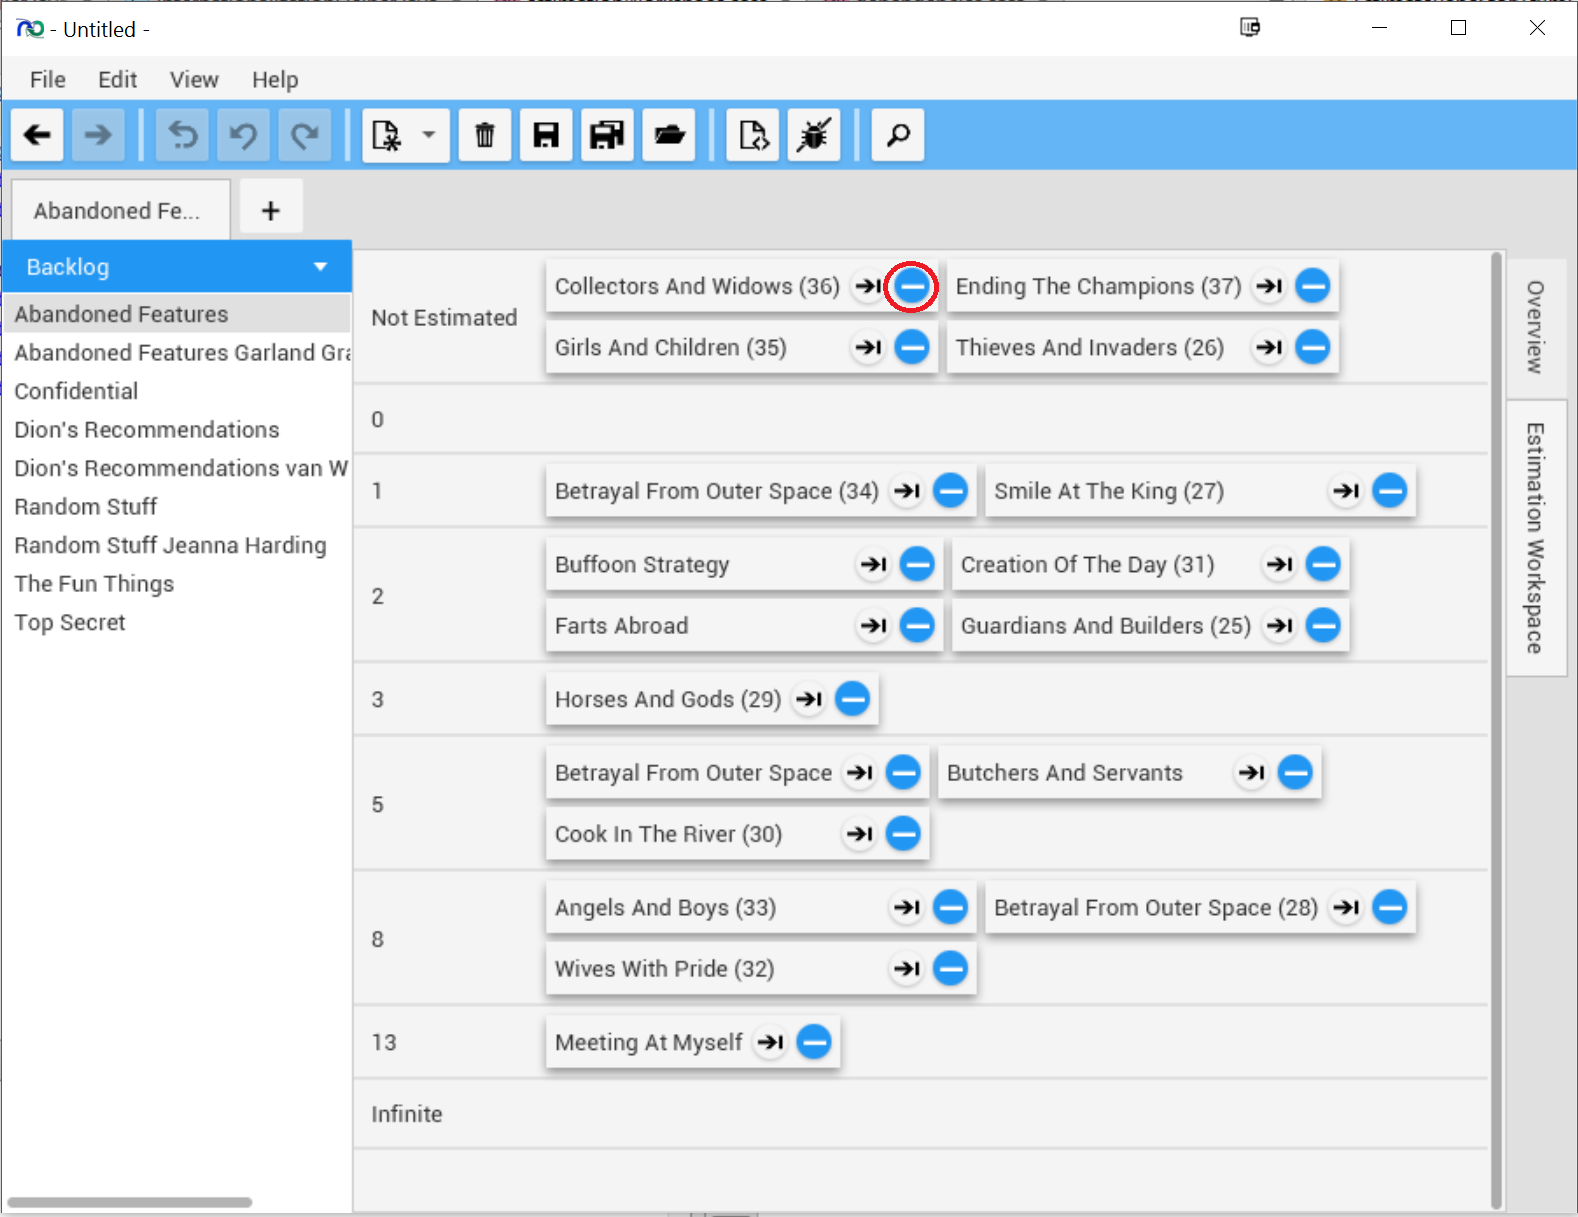
\includegraphics[width=\textwidth]{images/screenshots/estimationWorkspace3.PNG}
\caption{Removing stories from within the estimation workspace}
\label{fig:new_project}
\end{figure}

\pagebreak
Navigating to stories from within the workspace:
A story can be navigated to from within the workspace be selecting the button circled in red below.

\begin{figure}[H]
\centering
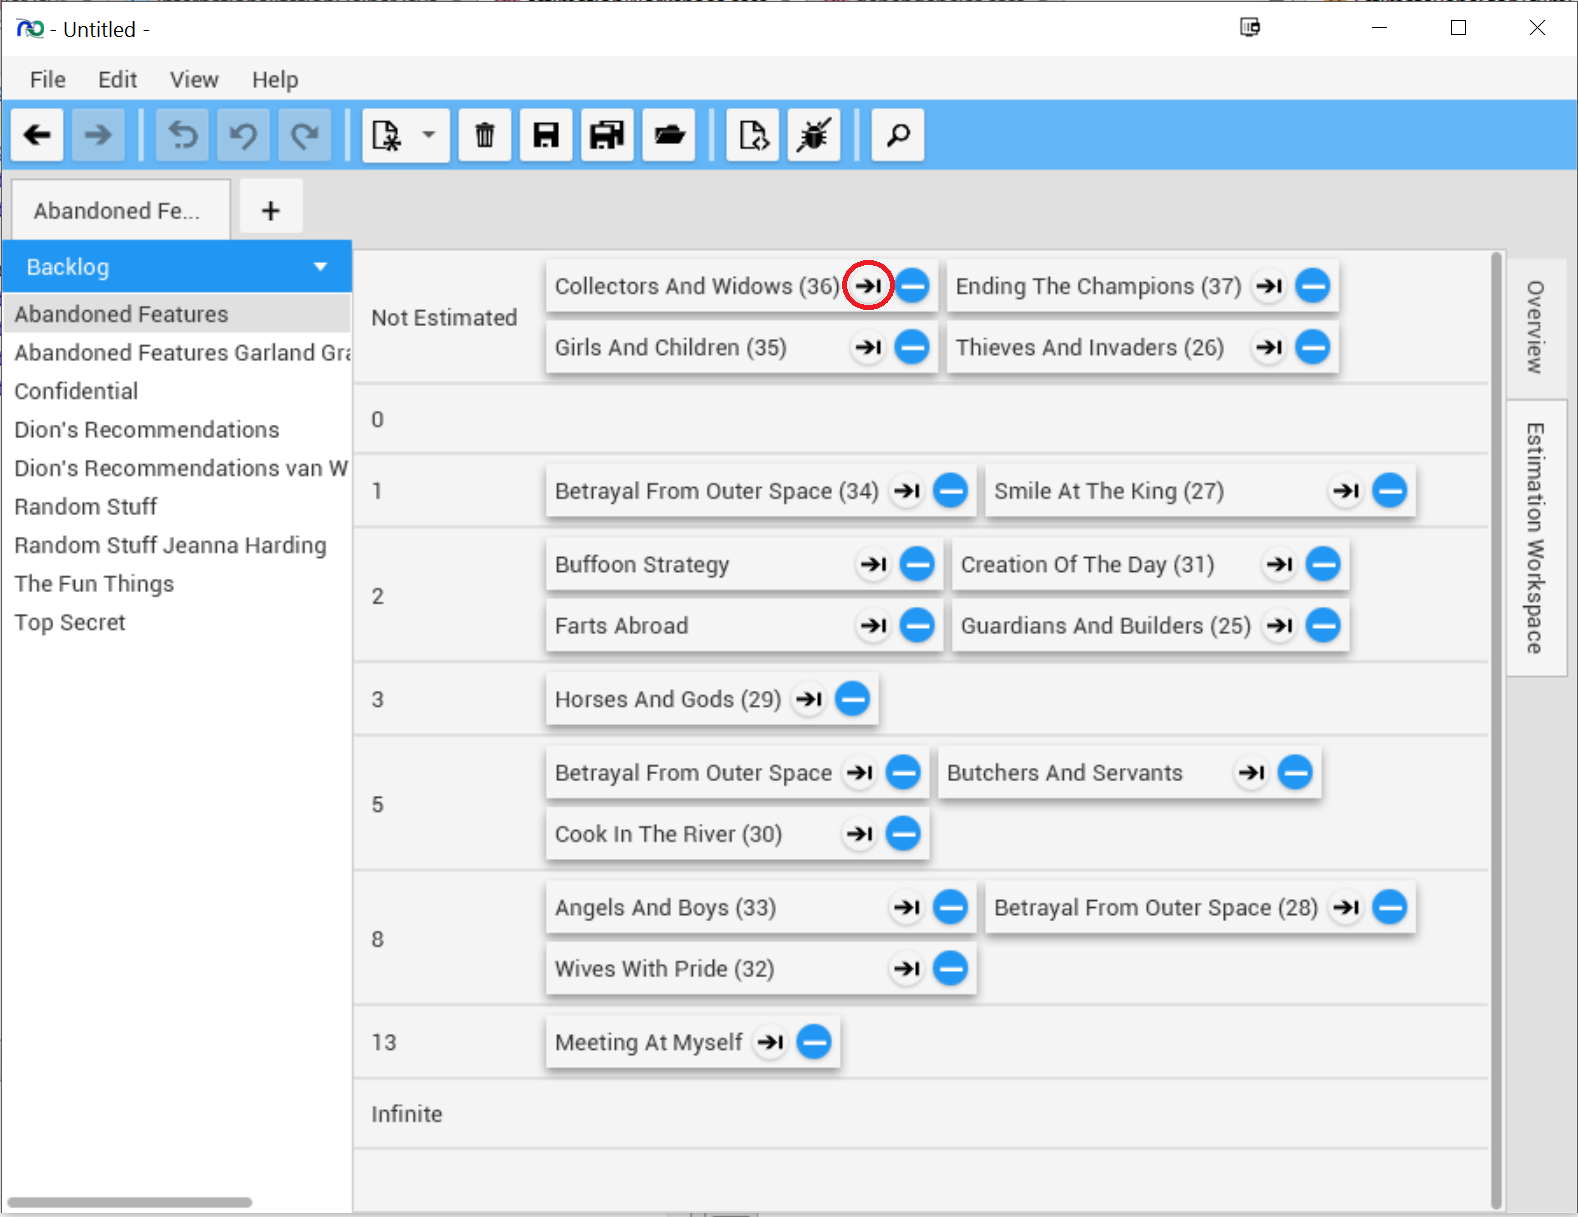
\includegraphics[width=\textwidth]{images/screenshots/estimationWorkspace4.PNG}
\caption{Navigate to a story from within the estimation workspace}
\label{fig:new_project}
\end{figure}








% A guide for deleting elements
\section{Element Deletion}

Elements can easily be deleted using the delete button found in the toolbar. You can also press delete with the item you want to delete selected. Following is a simple walk through for deleting an element.

First, choose the type of the element you wish to delete. This can be either Projects, Teams, People, Skills, Releases, Backlogs, Stories or Sprints and select it in the Display Choice Picker (circled below).

\begin{figure}[H]
\centering
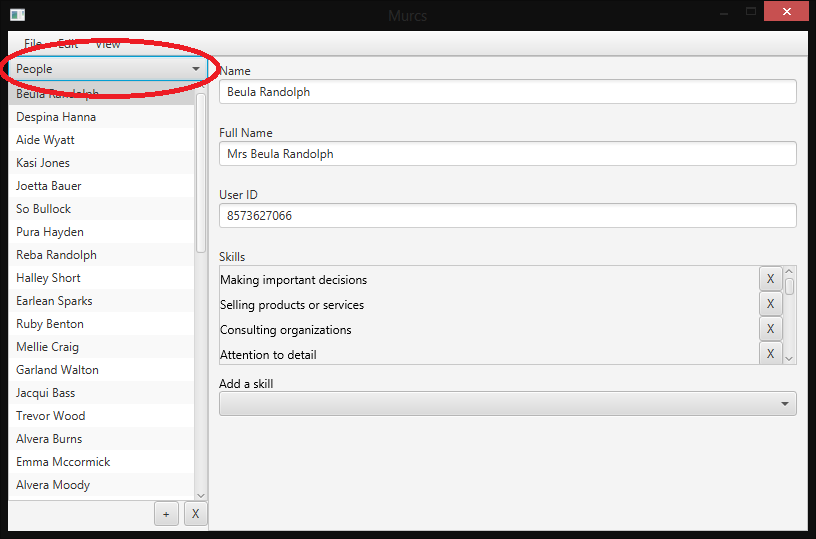
\includegraphics[width=\textwidth]{images/screenshots/deletion1.PNG}
\caption{The Display Choice Picker}
\label{fig:new_project}
\end{figure}

In our case, we've chosen to delete a person named Dion Vader. The next step is to select this person and press the delete button (circled below).

\begin{figure}[H]
\centering
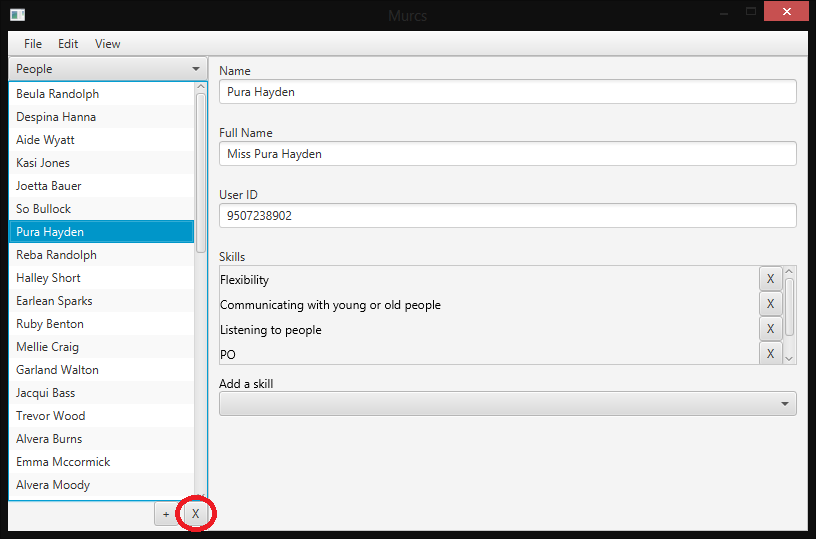
\includegraphics[width=\textwidth]{images/screenshots/deletion2.PNG}
\caption{The Delete Button}
\label{fig:new_project}
\end{figure}

The final step is to confirmation. You will be a presented with a message asking you if you are really sure you want to go through with a deletion along with a list of places that the element you are deleting is used. Press the 'Yes' button (circled) to go through with the deletion. If you've changed your mind you can click the 'No' button. 

\begin{figure}[H]
\centering
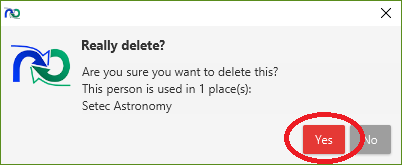
\includegraphics[width=\textwidth]{images/screenshots/deletion3.PNG}
\caption{The Confirmation Dialog. It seems Dion is part of a team named 'Setec Astronomy'}
\label{fig:new_project}
\end{figure}

Deleting Dion also removes him from anywhere else he may be used, so be careful!

If you've deleted something by mistake, don't worry! Deletions can be undone. Phew.

% A guide for reverting to a previous save
\section{Revert}

The program can be reverted to the last saved state by using revert. The button for which is located in the edit menu.
The revert functionality is only present if the program has been loaded from a file or saved at least once and there are unsaved changes.
Revert will ask for conformation before reverting because once the revert has been applied, any information not saved will be permanently lost.
Revert will also ask if you want to save changes as a new file before reverting.
\newline\newline


\begin{figure}[H]
\centering
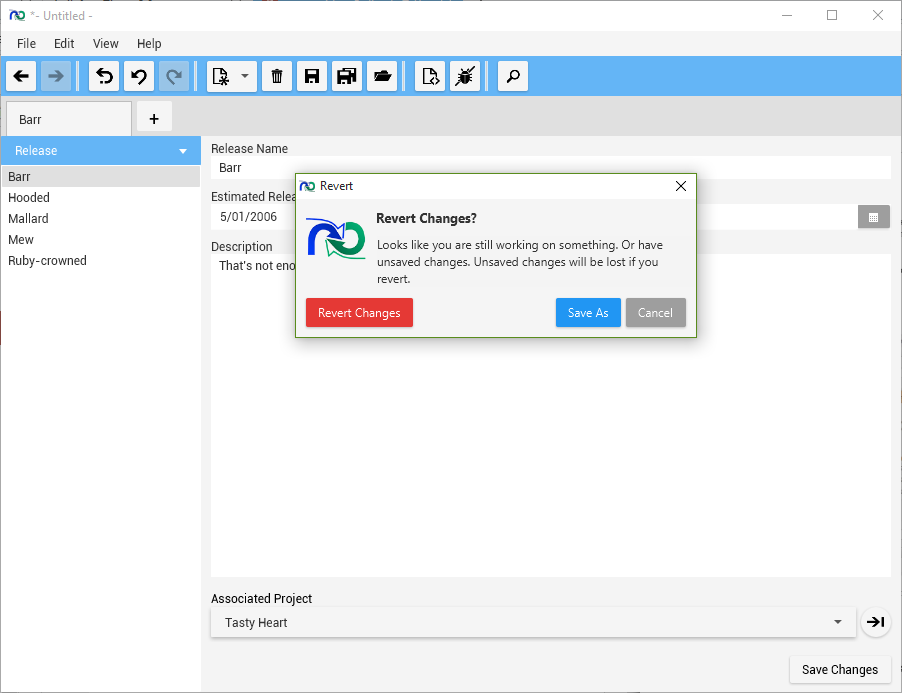
\includegraphics[width=\textwidth]{images/screenshots/revert1.PNG}
\caption{Reverting a change}
\label{fig:revert}
\end{figure}


% A guide for generating a XML report of the current state of the application
\section{Report Generation}

Generating Reports
\newline
If you should so wish it is possible to generate an XML version of the current state the application is in. This report will show you an overview of all your projects, teams, skills, people, team allocations etc so that you can get a general feel for everything in the current state.
\newline\newline
In order to generate this report all you need to do is click on File/Generate Report. When you do a dialog will appear asking where you would like to save the report and what file format you want to save it as (this defaults to XML, but if you want you can save it as a .report file). Once you have selected a location and pressed save then if you go to the location that you saved the report in and open the file you will have an XML representation of the file as shown in the diagram below.

\begin{figure}[H]
\centering
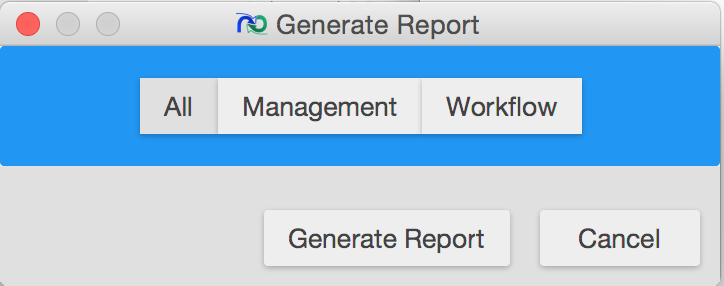
\includegraphics[width=\textwidth]{images/screenshots/report1.PNG}
\caption{The Display Choice Picker}
\label{fig:new_project}
\end{figure}

% A list of all the shortcuts in the application
\section{Shortcuts}

There are shortcuts for various commands in our application to make creating and other functionality easier. The list of shortcuts are given below:

\begin{itemize}
\item Open a .project file - CTRL + O
\item Save a .project file - CTRL + S
\item Save As a new .project file - CTRL + SHIFT + S
\item Generate a report - CTRL + G
\item Undo - CTRL + Z
\item Redo - CTRL + Y
\item Revert - CTRL + SHIFT + R
\item Show/Hide the side bar - CTRL + H
\item Start a new file - CTRL + N
\item Create a Project - CTRL + 1
\item Create a Team - CTRL + 2
\item Create a Person - CTRL + 3
\item Create a Skill - CTRL + 4
\item Create a Release - CTRL + 5
\item Create a Backlog - CTRL + 6
\item Create a Story - CTRL + 7
\item Go back - ALT + LEFT
\item Go forward - ALT + RIGHT
\item Add an item of the selected type in the display list - CTRL + '+' \(CTRL + SHIFT + '='\)
\end{itemize}


% A troubleshooting section detailing possible errors or problems that may occur, along with how to fix them
\section{Troubleshooting}

Try turning it on and off again. If that fails contact the developers at s301g1@cosc.canterbury.ac.nz

% A FAQ (Frequently Asked Questions)
\section{Frequently Asked Questions}

\newcommand{\faqentry}[2]{\textbf{Q. #1}\\  \textbf{A.} \textit{#2}\vspace{0.5cm}}


\faqentry{How do I make it work?}{Run it from the jar or compile it from the source code}

\faqentry{Can I make it generate random information to use as a starting base?}{Yes. Simply add the argument debug (with optional low, medium high afterwards) when you run the jar and it will automatically generate some information for you to use. This may be a bit more technical than most people will want. It is also not supported by us so if it goes wrong you can't blame us as you've been warned.}

\faqentry{What happens with my old projects?}{Currently they will not be loaded at all and a dialog will appear informing you to open it with the same version of the application that you created it with. We are working towards having support for all old version of .project files.}

\faqentry{
Are there any bugs?
}
{
Yes. The current bugs that we know of include: \newline \begin{itemize}
  \item People can not be unassigned from roles within teams, they can only be replaced.
  \item When a creation form detects an error in input it isn't always very obvious as sometimes it is hidden.
  \item When creating a project if a invalid work allocation is added, the project can not be created.
  \item Status reports are not pretty printed correctly.
  \item (Minor or unnoticeable) When using the debug option generated objects like people may end up being assigned to multiple teams which they shouldn't be able to do.
\end{itemize}
}

\end{document}
